\section{The new DAC System}
\label{sec:mywork}

In this section, my work on the DAC system and ZEF shall be elaborated more. The direct air capture unit (DAC) in the ZEF microplant captures $CO_2$ from the atmosphere using the polyethyleneimine (PEI). The following are the different stages in the DAC System which will be looked at in these subsections given below :

\subsection{The DAC sub-stages}

The DAC system in ZEF 5 which we had worked on and made contains 2 sub - systems namely absorption unit and desorbtion unit. The sub - systems are elaborated below. 

\subsubsection{Stage 1 - Absorption}
PEI is exposed to air by exposing it to the atmosphere and using a high power suction fan creating a cross current flow between the flow of air and the flow of PEI. $CO_2$ is absorbed into the PEI using chemisorption. The PEI containing $CO_2$ is collected in the collector and then passed to the desportion chamber. 

\subsubsection{Stage 2 - Desportion}

The PEI containing absorbed $CO_2$ is passed into a vacuum chamber that maintains the pressure at near vacuum conditions using a 4 - stage compressor. The vacuum chamber is also heated to elevated temperature using heating catridges. The temperature is controlled using a PID controller that turns the heater on or off till it reaches a desired set temperature which is at about 100 \degree C. The temperature isn't supplied more that 120 \degree C as it is found from literature by the ZEF I team that PEI starts to degrade rapidly at that temperature. 
\bigbreak \noindent
It is also found from literature study by ZEF II team that oxygen degrades PEI at elevated temperatures quite rapidly and this is leads to undesirable effect. Hence, we use a vacuum conditions to faciliate the desportion process. The desorbed gases containing $CO_2$, $H_2O$ and other gases is passed out of the compressor at 50 bar.
\bigbreak \noindent
After the gases have been desorbed from the heated PEI. It PEI is passed down into a PEI pump that supplies PEI back into the absorber subsystem. The absorber subsystem takes the PEI into the manifold that splits the PEI into 8 different distributors. The distributors are designed in such a way that maximum PEI is exposed to the atmosphere for direct air capture. Thereby, making the whole system a continuous system based on the designs of ZEF IV which is summarized in Section \ref{sec:zef4}.

\subsection{Sprint 1 - $2^{nd}$ September to $23^{rd}$ September}
\label{sec:sprint1}

Based on the designs and first model fabricated by the ZEF IV team which has been elaborated on in Section \ref{sec:zef4}. During the $1^{st}$ sprint period of my internship in ZEF IV which spanned from $2^{nd}$ September to $23^{rd}$ September I took sometime to learn about 3D printing and about the DAC system and the onboarding process of ZEF. Then, I had fabricated the DAC system V1.1 absorber and column.  

\subsubsection{DAC V1.1 system absorber}


I was tasked to fabricate the DAC V1.1 System. The system had some minor changes compared its predecessor such as some changes in the distributor design. The inlet nozzle changed orientation. The outer casing of the DAC absorber column design was also changed inorder to make it more easy to remove or add the DAC flow channels into the DAC absorber column. 
\bigbreak

\begin{figure}[H]
    \centering
    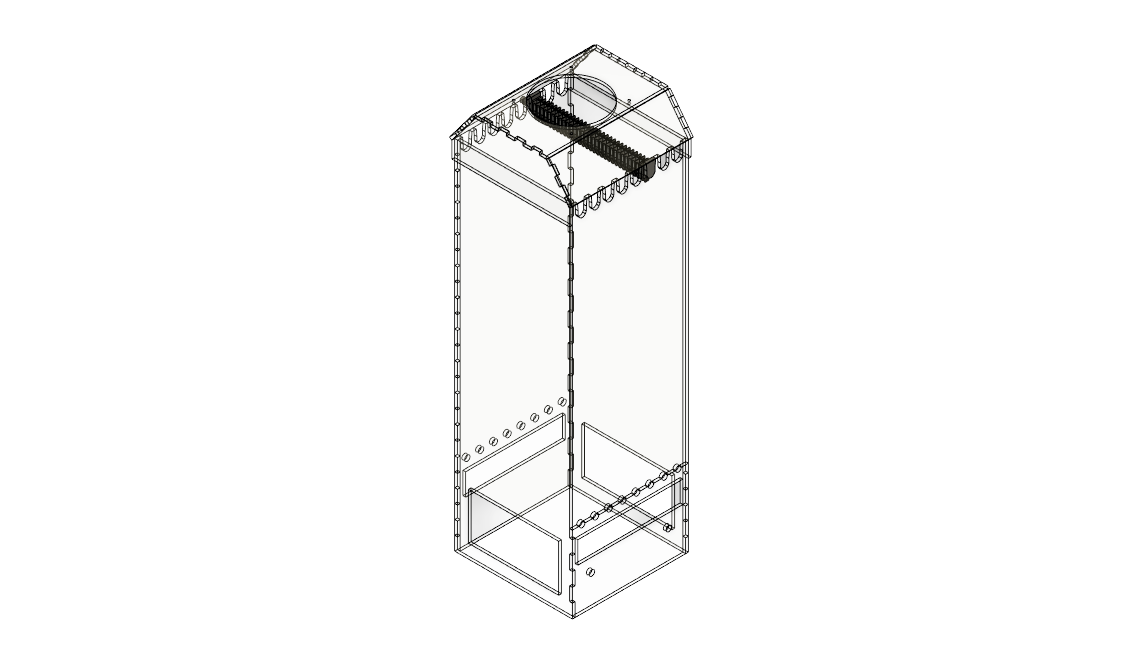
\includegraphics[scale = 0.4]{images/mywork/Sprint1/Column.png}
    \caption{The new DAC PMMA columns of ZEF}
    \label{fig:daccolumn}
\end{figure}

\begin{figure}[H]
\centering
\begin{minipage}{.5\textwidth}
  \centering
  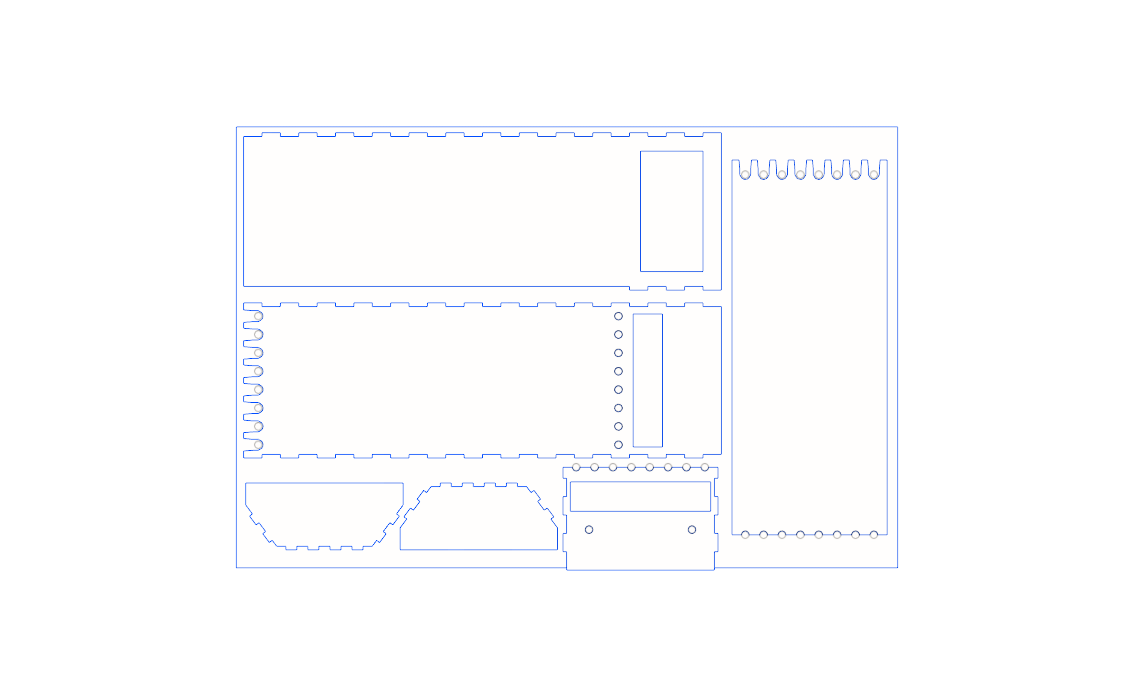
\includegraphics[width=\linewidth]{images/mywork/Sprint1/Lasersheet1.png}
  \captionof{figure}{PMMA sheet 1}
  \label{fig:pmma1}
\end{minipage}%
\begin{minipage}{.5\textwidth}
  \centering
  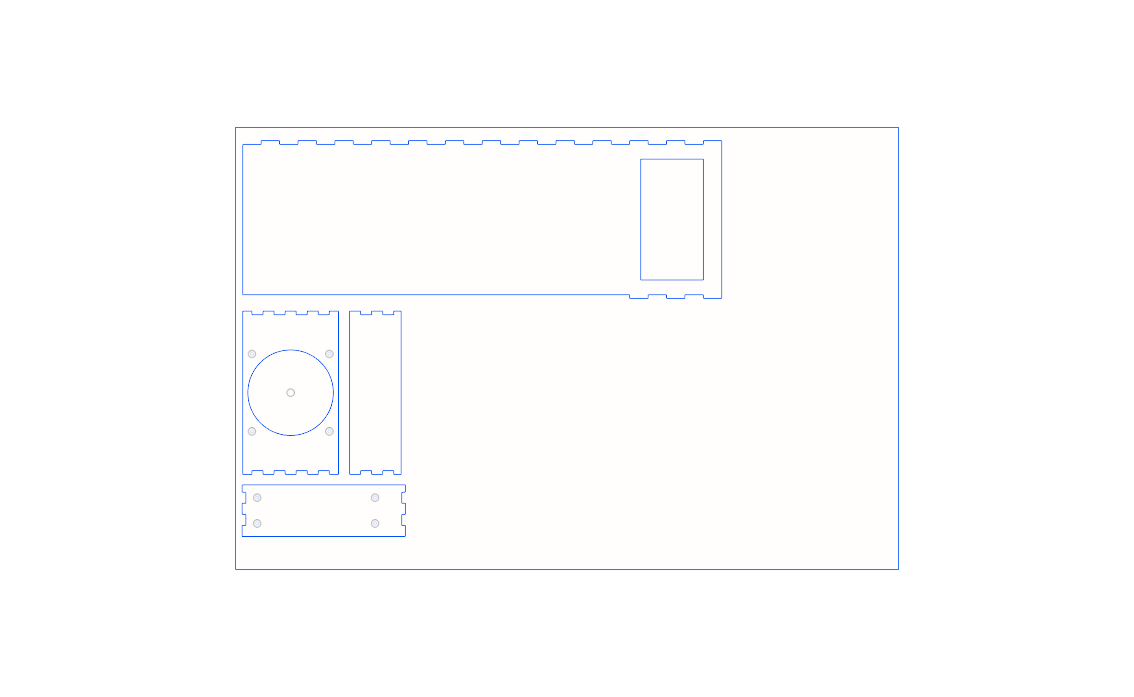
\includegraphics[width=\linewidth]{images/mywork/Sprint1/Lasersheet2.png}
  \captionof{figure}{PMMA sheet 2}
  \label{fig:pmma2}
\end{minipage}
\end{figure}

First, the DAC column which can be seen in full assembly in Figure \ref{fig:daccolumn} was fabricated using PMMA sheets which were purchased from Laserbeest. Based on the designs shown in Figure \ref{fig:daccolumn}, Jan had designed the PMMA sheets for the laser cutting for the assembly parts for the DAC column as well before my internship had begun. The PMMA sheet designs can be seen in Figure \ref{fig:pmma1} and Figure \ref{fig:pmma2}. The PMMA sheets were lasercut based on the above designs in the Industrial Department of TU Delft which took not more than 10 minutes. 
\bigbreak
The laser cut parts were then assembled in the ZEF workshop using duct tape as it still wasn't a final design. The PMMA cut parts fit perfectly with each other and can be seen in the Figure \ref{fig:pmmaass1} which contains the top hat for the fan that sucks air out of the DAC column to the atmosphere and Figure \ref{fig:pmmaass2} is the DAC column without the top hat, we can also see the DAC distributor fitting snuggly in the slots.  


\begin{figure}[H]
\centering
\begin{minipage}{.5\textwidth}
  \centering
  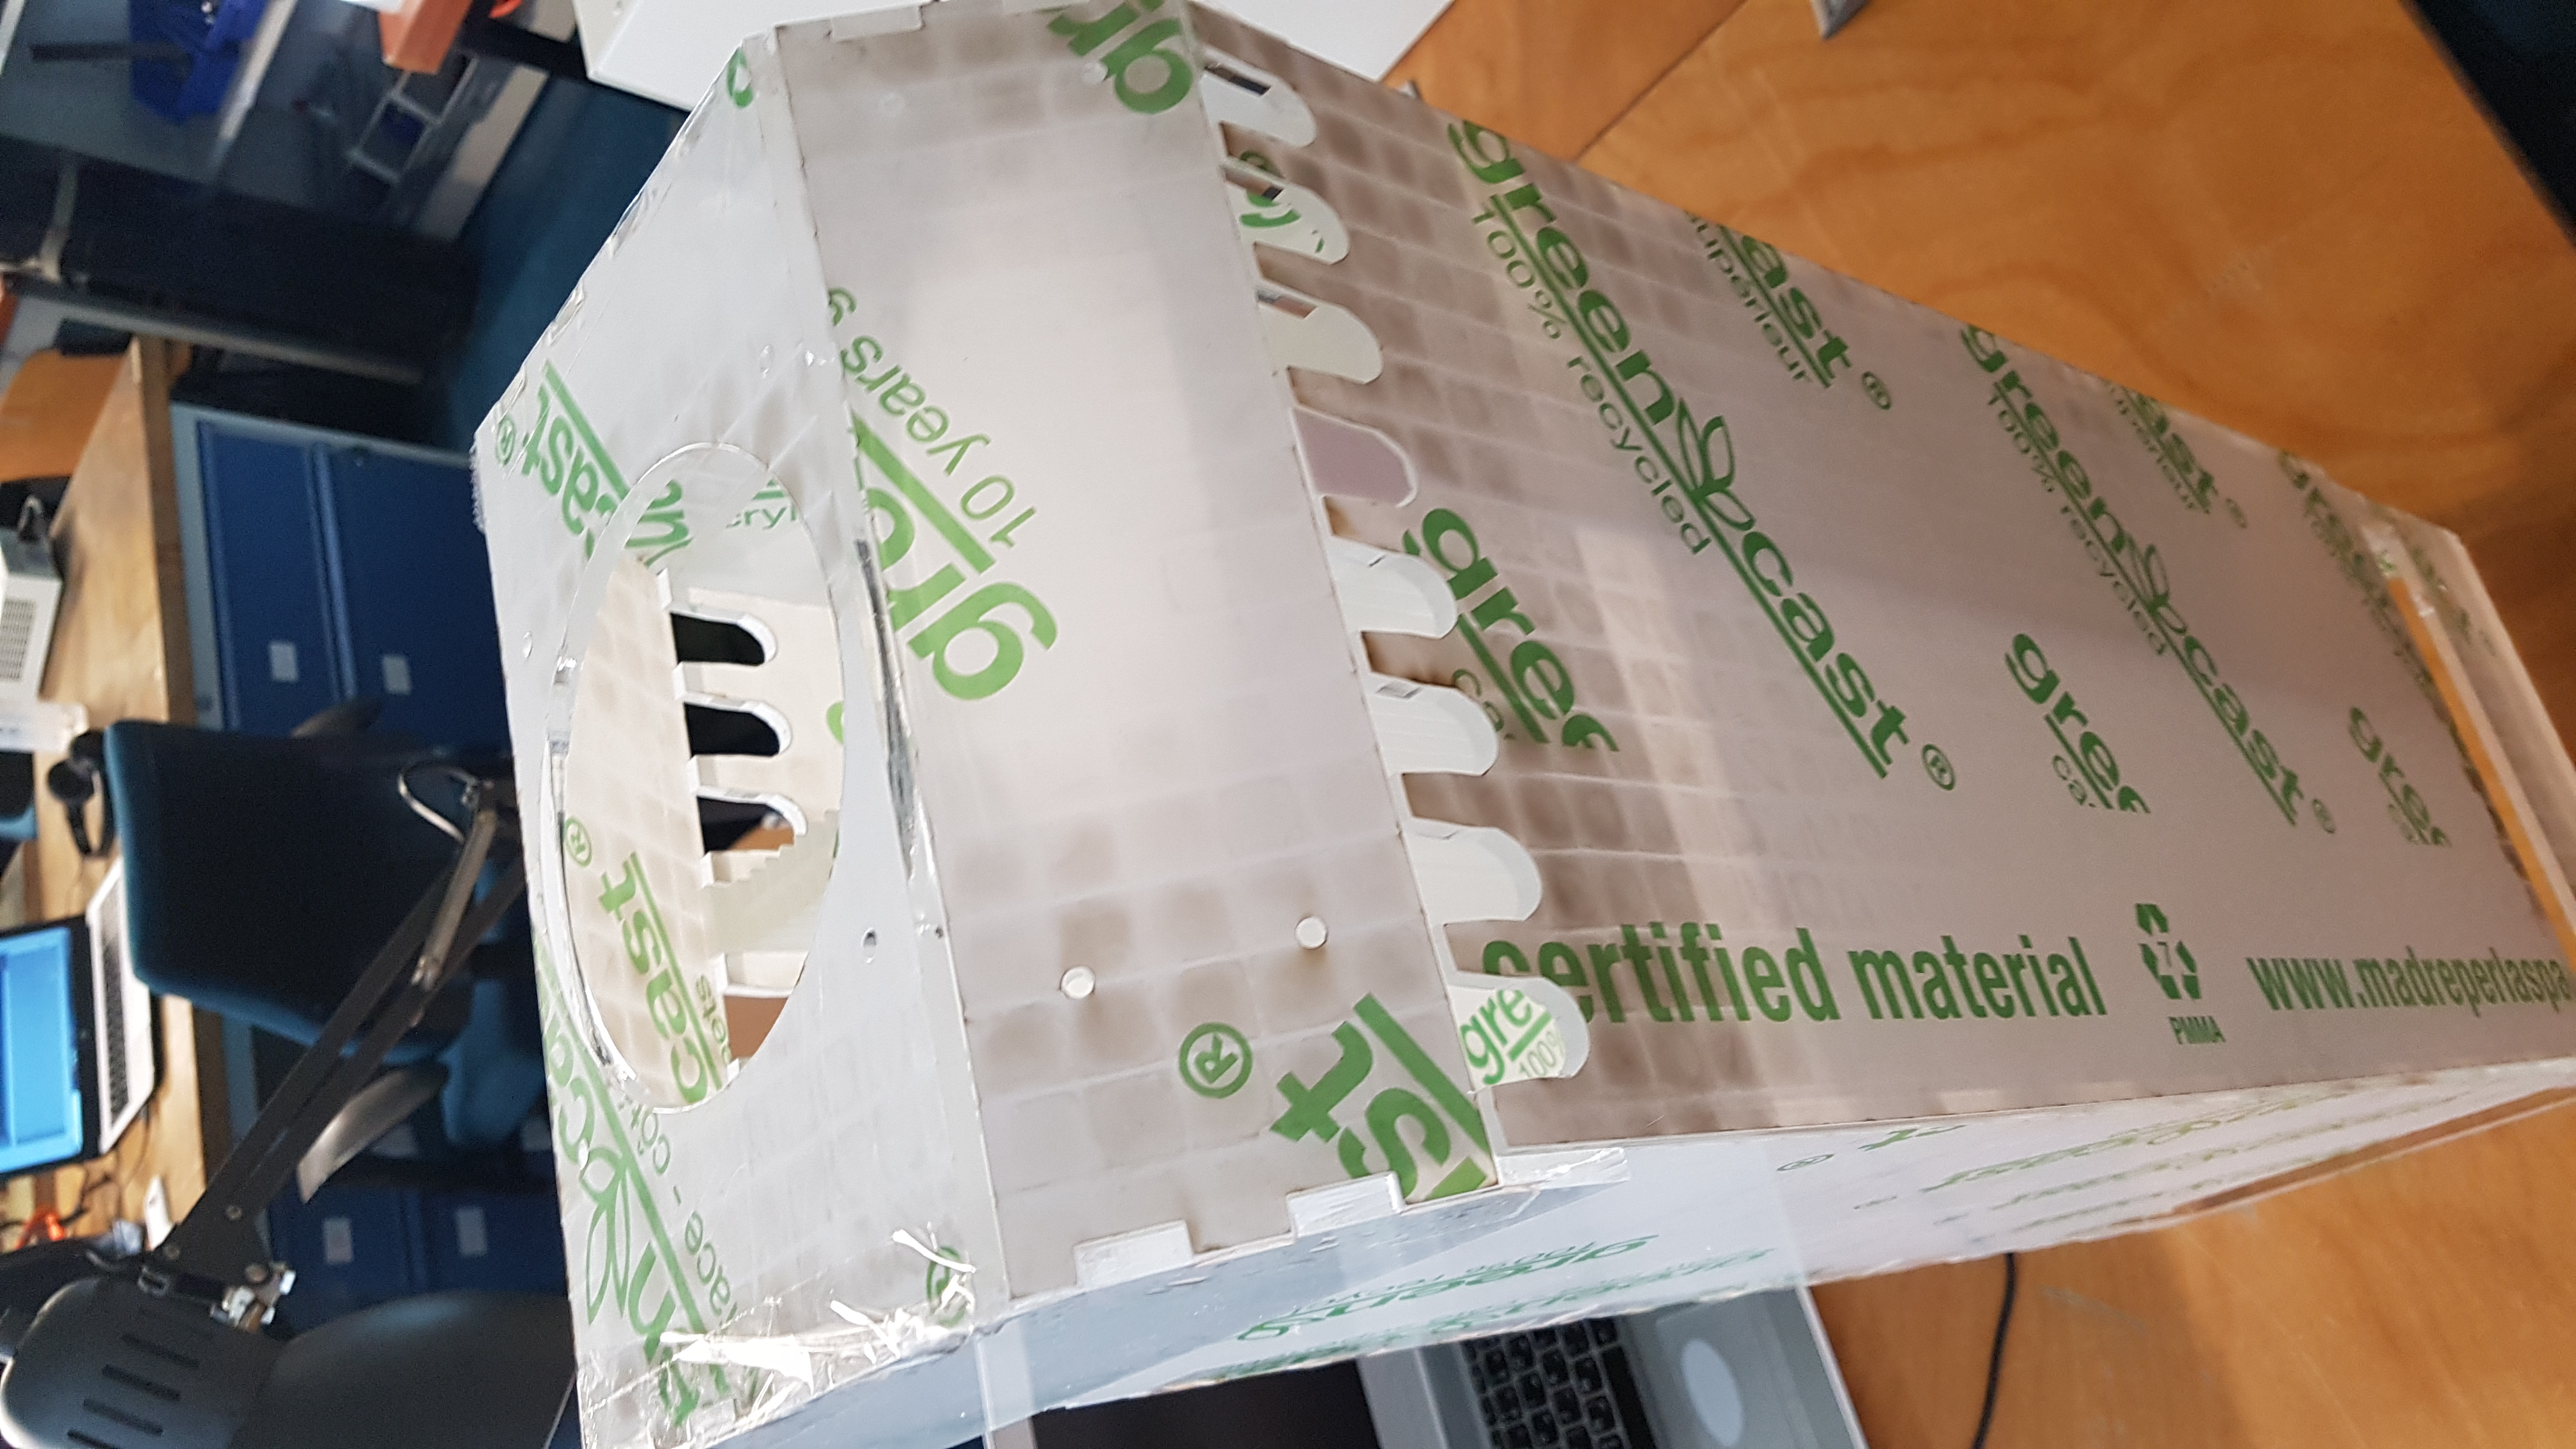
\includegraphics[width=\linewidth,angle = 270]{images/mywork/Sprint1/PMMAAssembled.jpg}
  \captionof{figure}{DAC column with top hat}
  \label{fig:pmmaass1}
\end{minipage}%
\begin{minipage}{.5\textwidth}
  \centering
  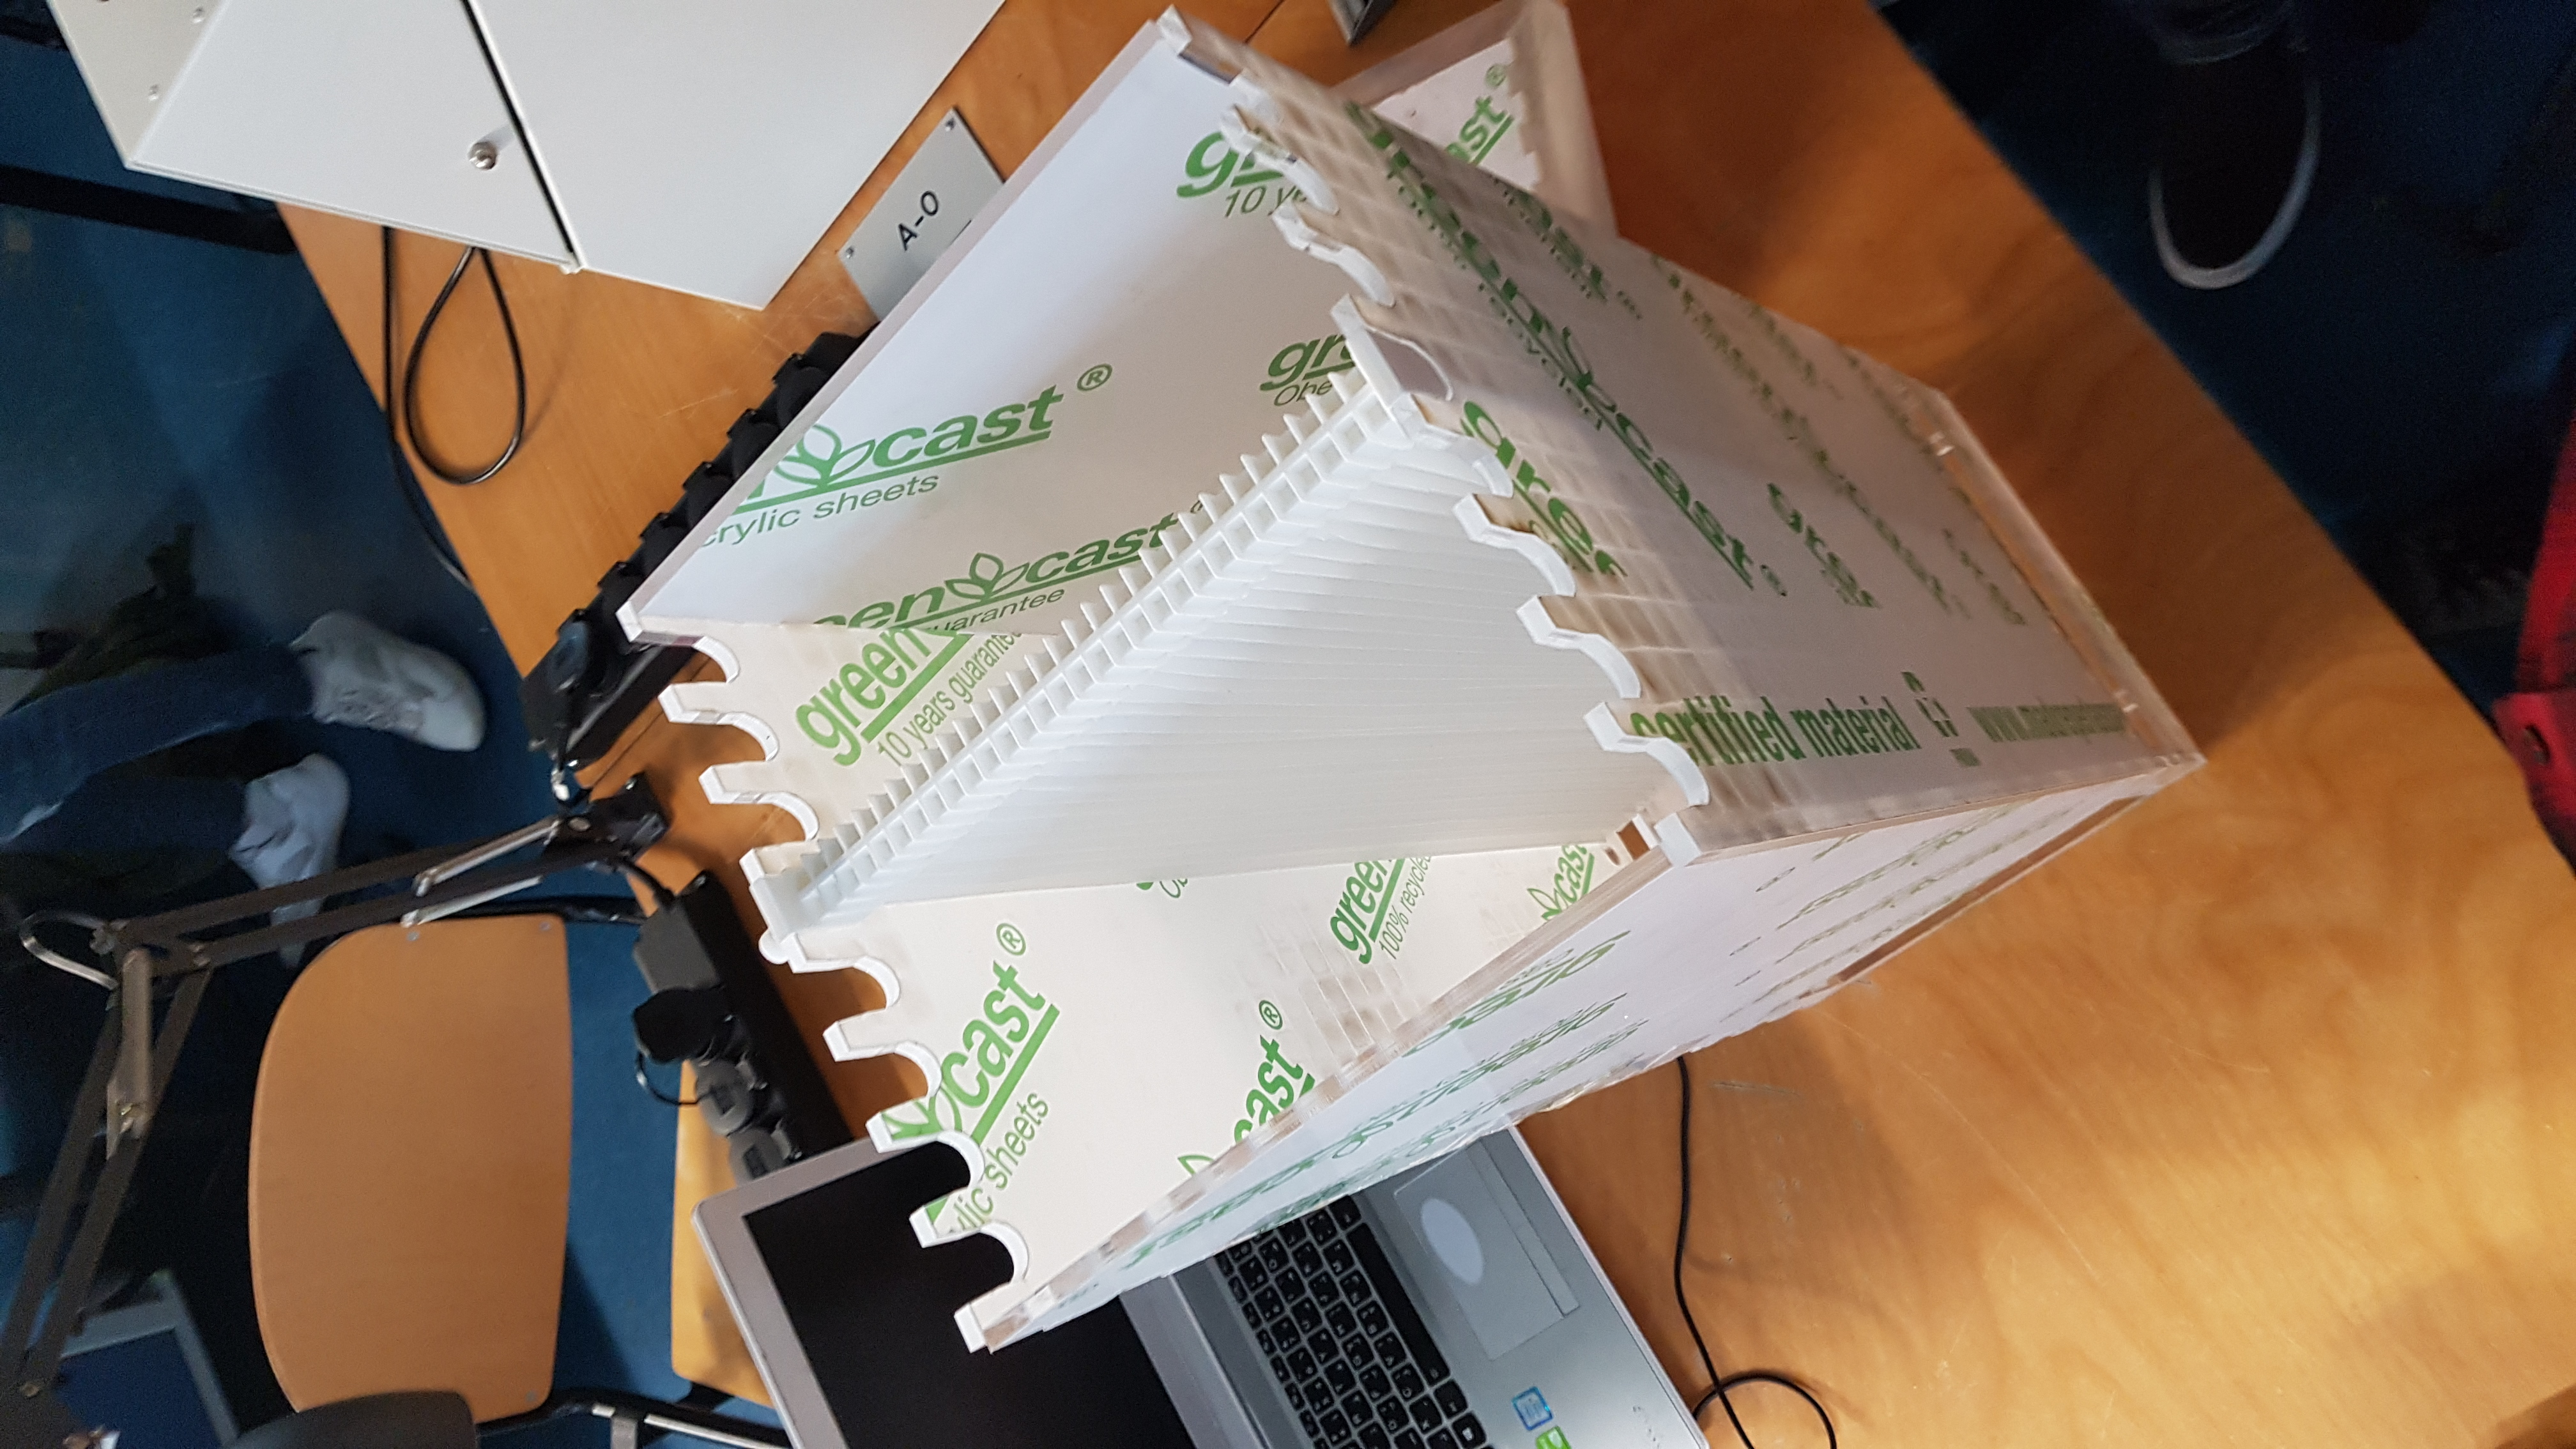
\includegraphics[width=\linewidth, angle = 270]{images/mywork/Sprint1/AssembledPMMA.jpg}
  \captionof{figure}{DAC column with distributor}
  \label{fig:pmmaass2}
\end{minipage}
\end{figure}

Based on ZEF IV designs for the distributor and manifold minor design changes were made inorder to make some parts more robust. The parts were manufactured using 3D printing with print material used as Polylactide (PLA). Since, the old DAC collectors had no design changes and weren't broken. We continued to use them with the new system as well, which were 3D printed by the previous team as well. The printer used was a Utimaker 2+ which was made with leaktight settings (high infill \% and very low layer height) in the Ultimaker Cura software for 3D printing. 

\begin{figure}[H]
\centering
\begin{minipage}{.5\textwidth}
  \centering
  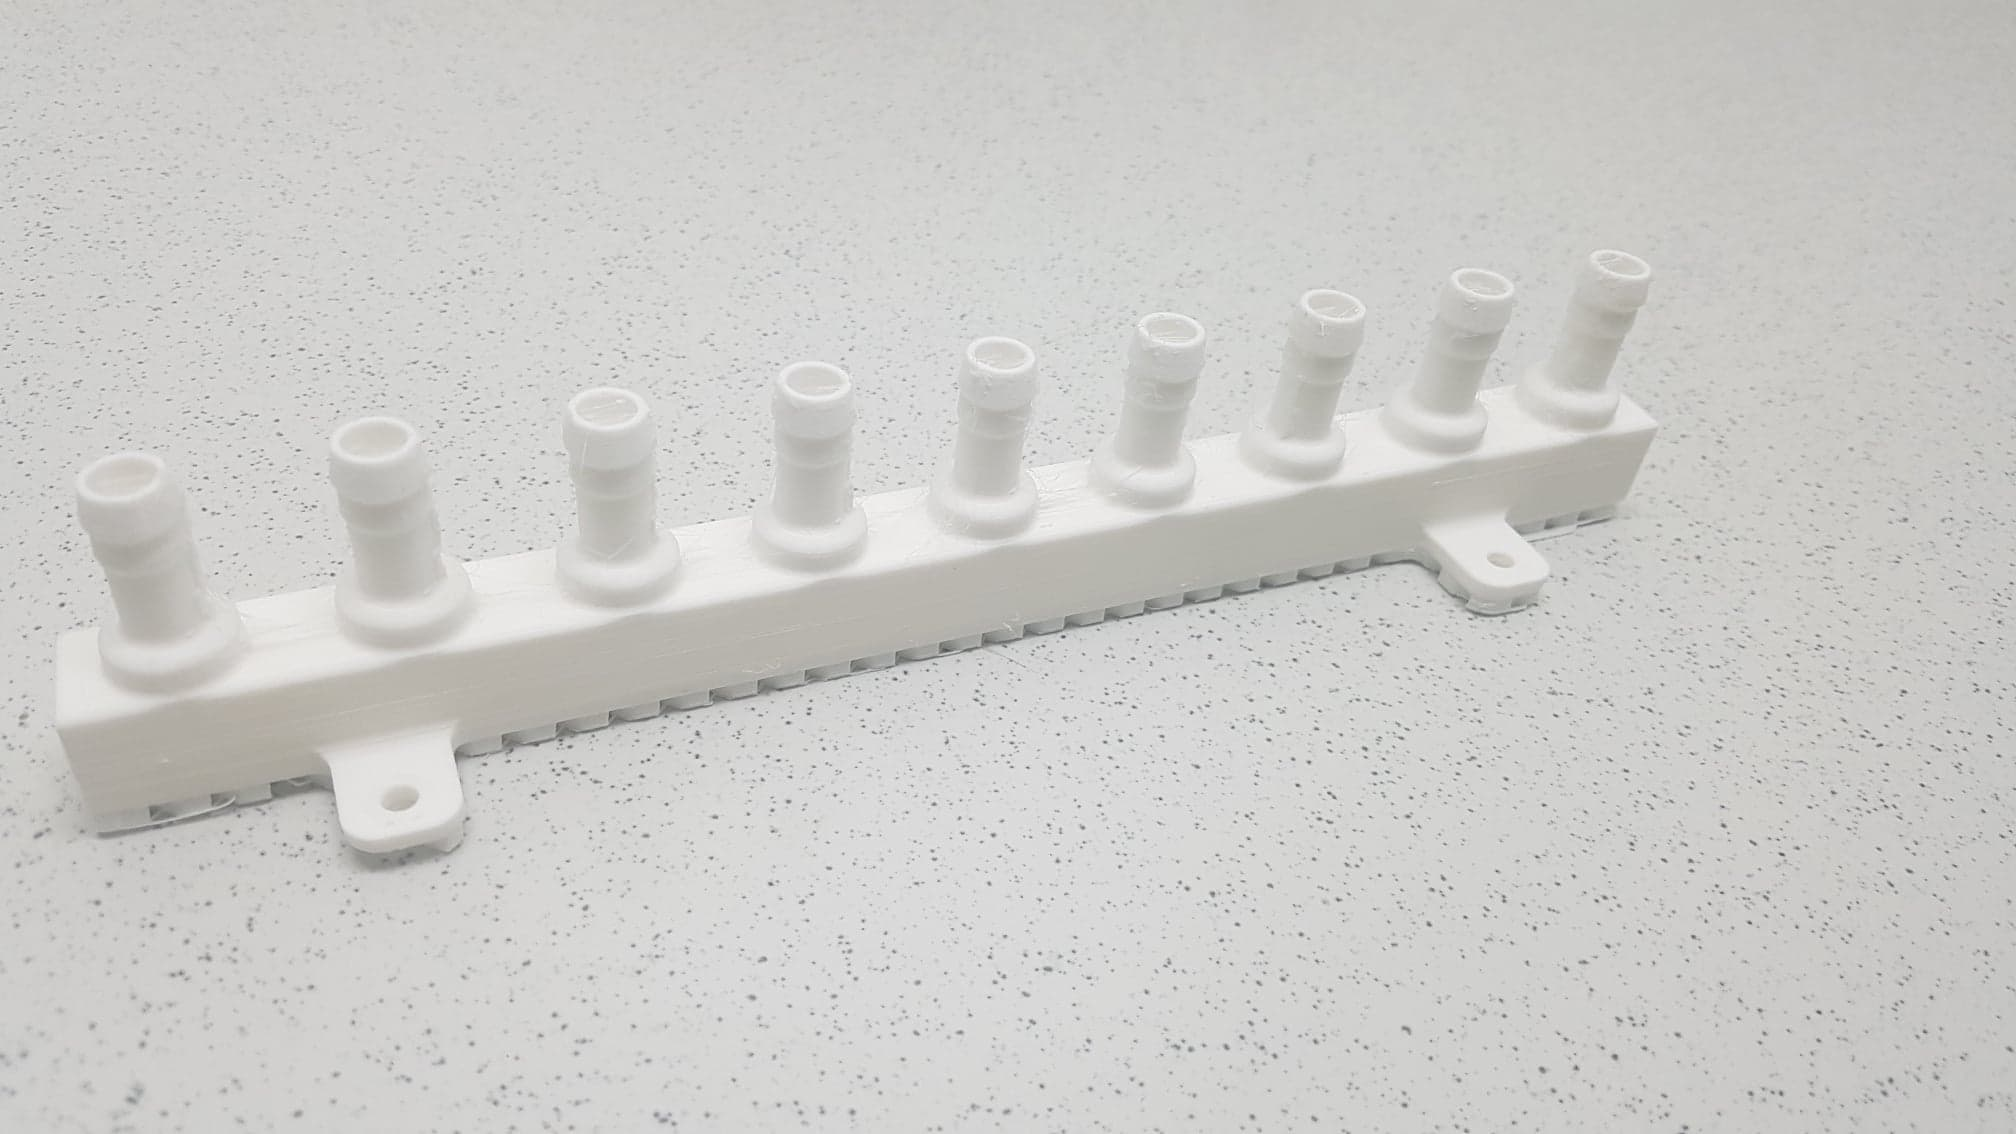
\includegraphics[width=0.9\linewidth]{images/mywork/Sprint1/Manifold.jpg}
  \captionof{figure}{3D DAC manifold}
  \label{fig:3Dmanifold}
\end{minipage}%
\begin{minipage}{.5\textwidth}
  \centering
  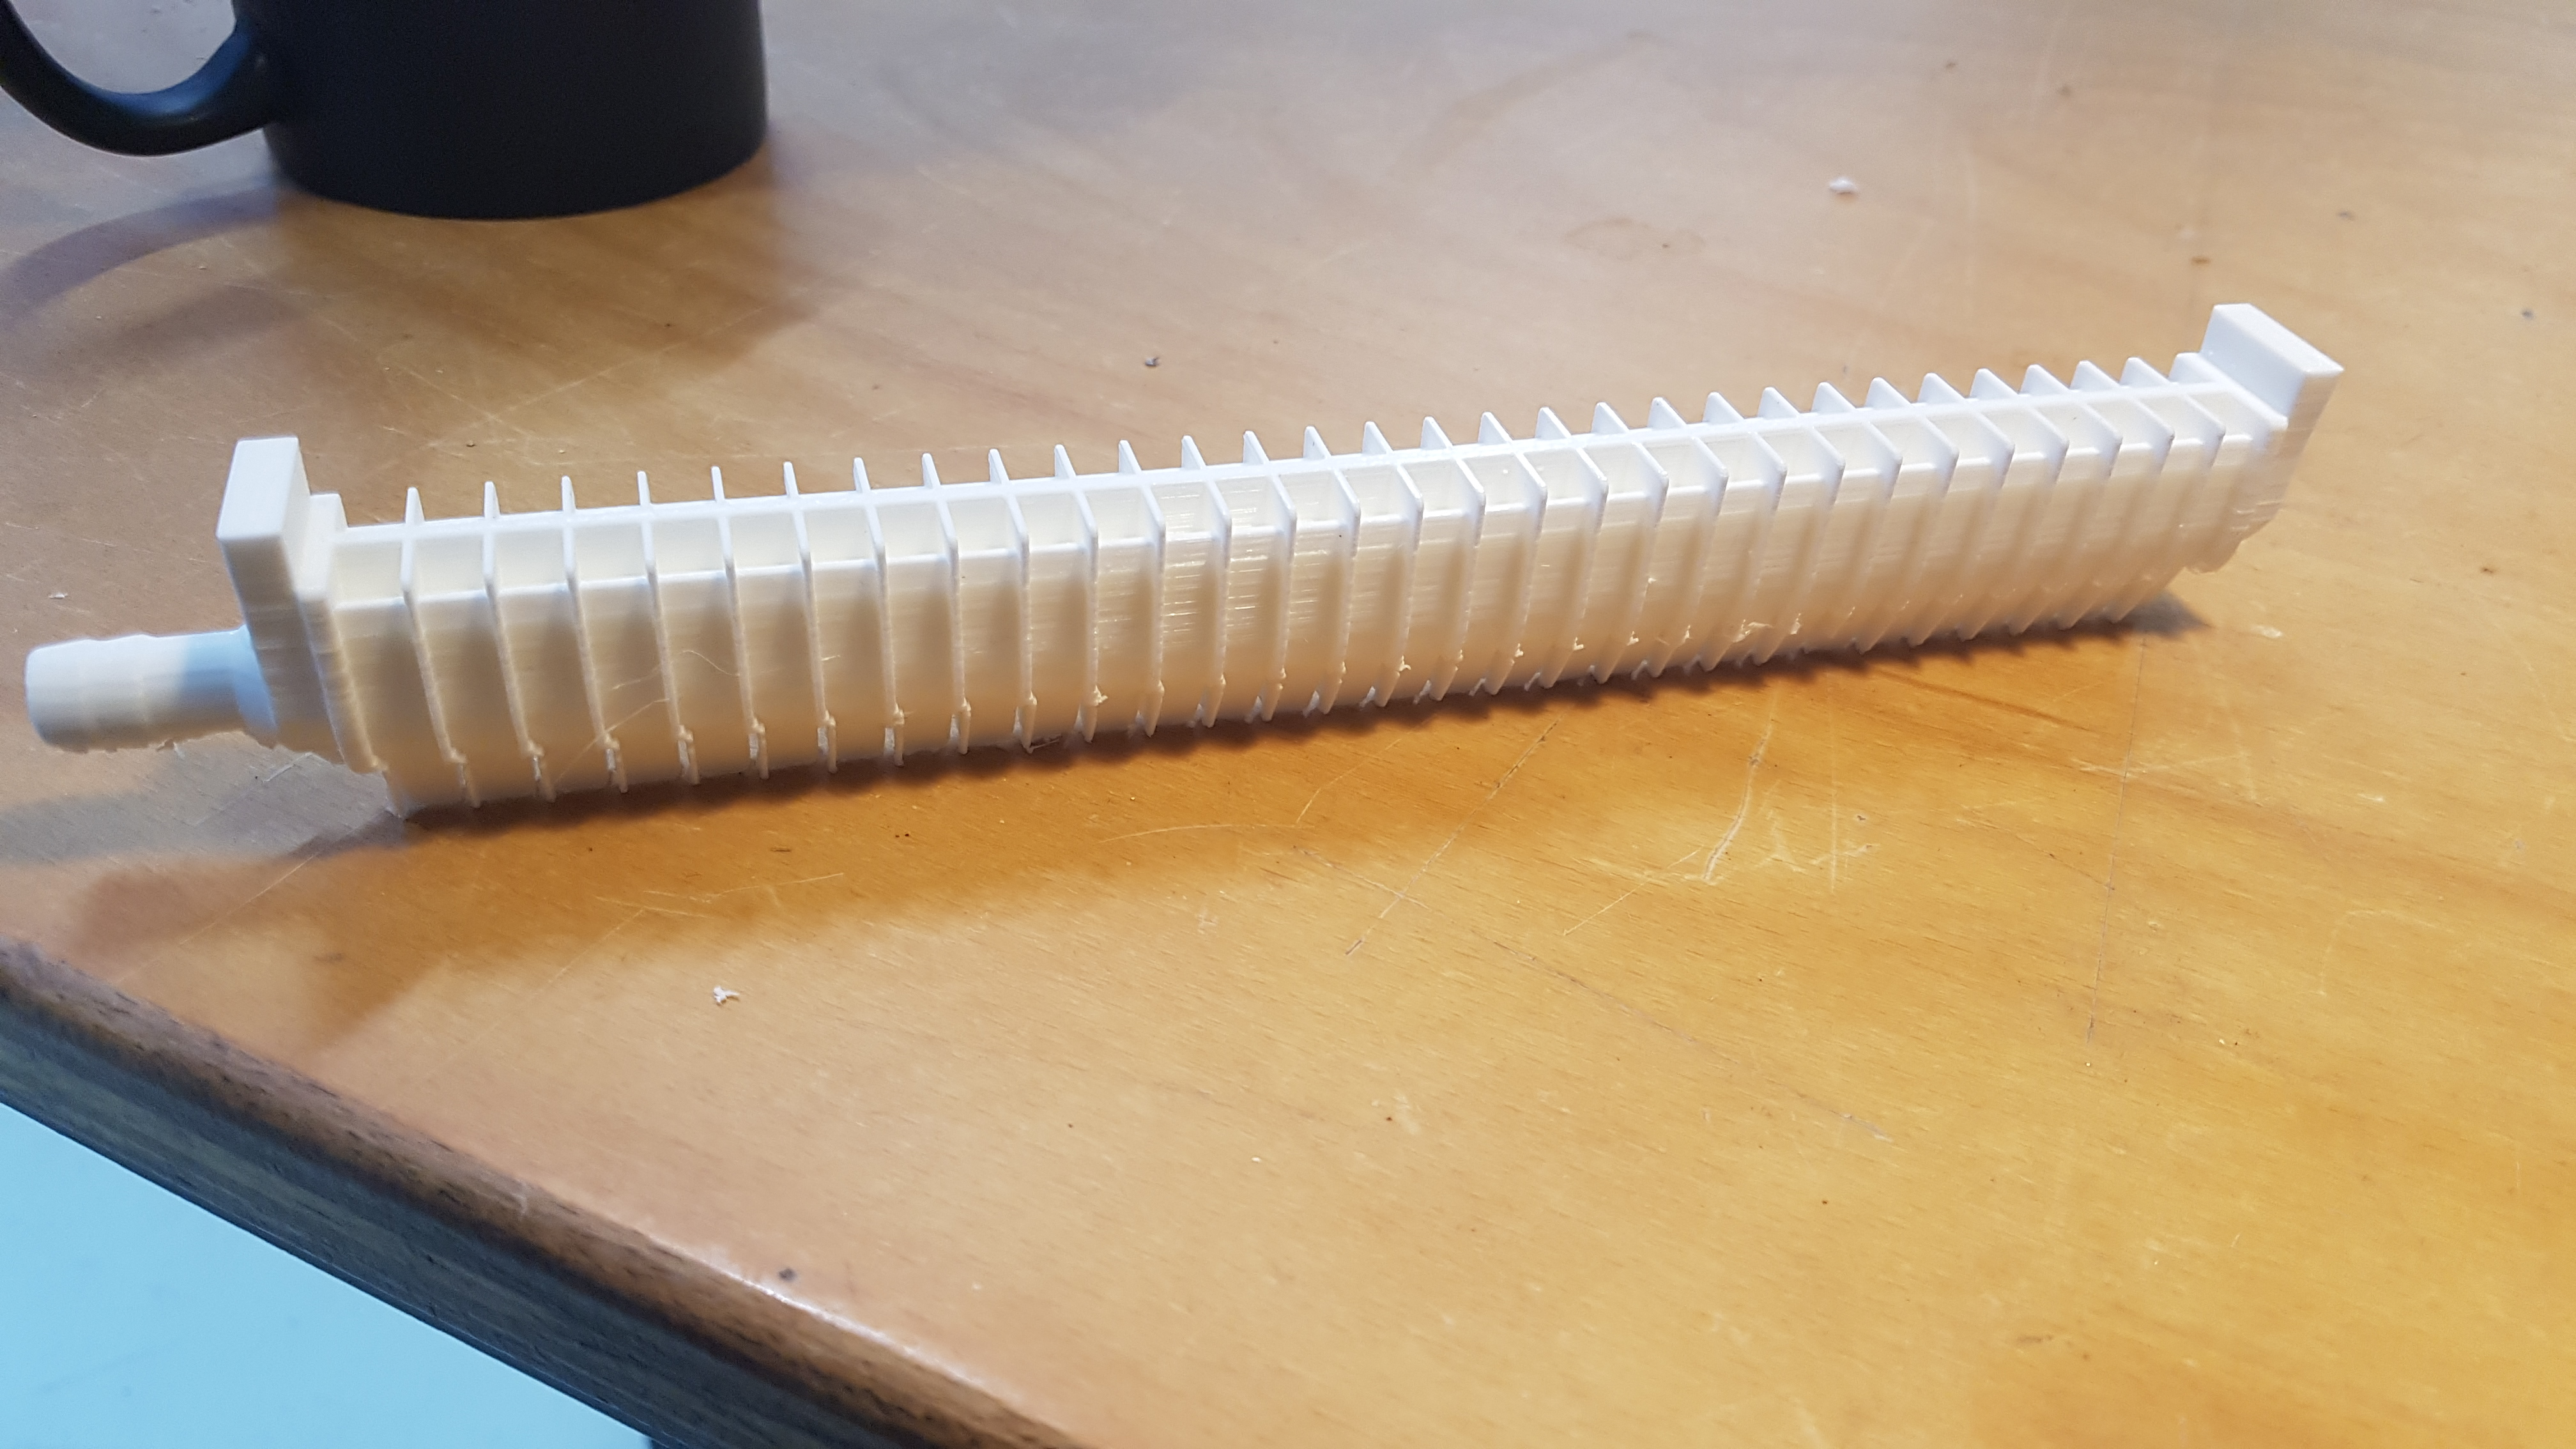
\includegraphics[width=0.9\linewidth]{images/mywork/Sprint1/Distributor.jpg}
  \captionof{figure}{3D DAC distributor}
  \label{fig:3Ddistributor}
\end{minipage}
\end{figure}

In Figures \ref{fig:3Dmanifold} we can see the final 3D printed DAC manifold and in Figure \ref{fig:3Ddistributor} we can see the final 3D printed distributor. It can be seen that in the Figure \ref{fig:pmmaass1} that there is a list of components needed for the DAC absorber column: 
\begin{itemize}
    \item DAC distributors x8 
    \item DAC manifold x1 
    \item DAC collectors x8 
    \item DAC flow channels x8
    \item DAC collector bucket x1 
    \item Silicon connecting pipes
\end{itemize}

Since, we needed a large number of DAC distributors and each 3D print take about 24 hours. We had to utilize the 3D printers at Industrial design department of TU Delft. For the DAC flow channels, we used the DAC system V1.0's flow channels itself and it had the same required specifications. The channels were ordered from an external company called Windowprint. The channel is cut across its width and halved. It is then cut to the required shape and stuck to each other using a plastic sealing machine (mostly used to seal sandwich bags). Finally, they are fitted into the DAC distributor and placed inside the DAC absorber column with the DAC collectors. The final assembly of the DAC absorber column can be seen in Figure \ref{fig:absorber} below.  

\begin{figure}[H]
    \centering
    \includegraphics[scale = 0.155]{images/mywork/Sprint1/absorber.png}
    \caption{Complete DAC absorber column}
    \label{fig:absorber}
\end{figure}

\subsection{Sprint 2 - $23^{rd}$ September to $14^{th}$ October}
\label{sec:sprint2}

During the sprint 2 period of my internship spanning from $23^{rd}$ September to $14^{th}$ October. I turned my attention toward the desorbtion part and running the DAC system V1.1 as one whole unit and getting the pumps and compressor to run using an Arduino 2560MEGA.  

\subsubsection{DAC V1.1 system desorber}
\label{sec:faultycomp}

The desorber unit which consists of a desorbtion chamber that heats the PEI to a set temperature (normally set to 80 \degree C) which can be controlled using temperature sensors and arduino code. The PID heater controller arduino code can be further examined in Appendix \ref{ap:arduino}. In the previous Section \ref{sec:zef4}, we have seen that they have already fabricated and used the desorbtion chamber and a vacuum pump to suck the absorbed $CO_2$ from the heated PEI in the desorbtion chamber using Pressure swing desorbtion. The desorber unit also consists of the PEI pump which was inoperational due to lose connections and incorrect code. The motor is now operational with proper connections in the bread board and with the the new "Motor starting" arduino code which starts the servo motor and sets the RPM of the motor as well, refer Appendix \ref{ap:arduino} for further examination. %refer picture in the zef4 section and explain about it

\begin{figure}[H]
\centering
\begin{minipage}{.5\textwidth}
  \centering
  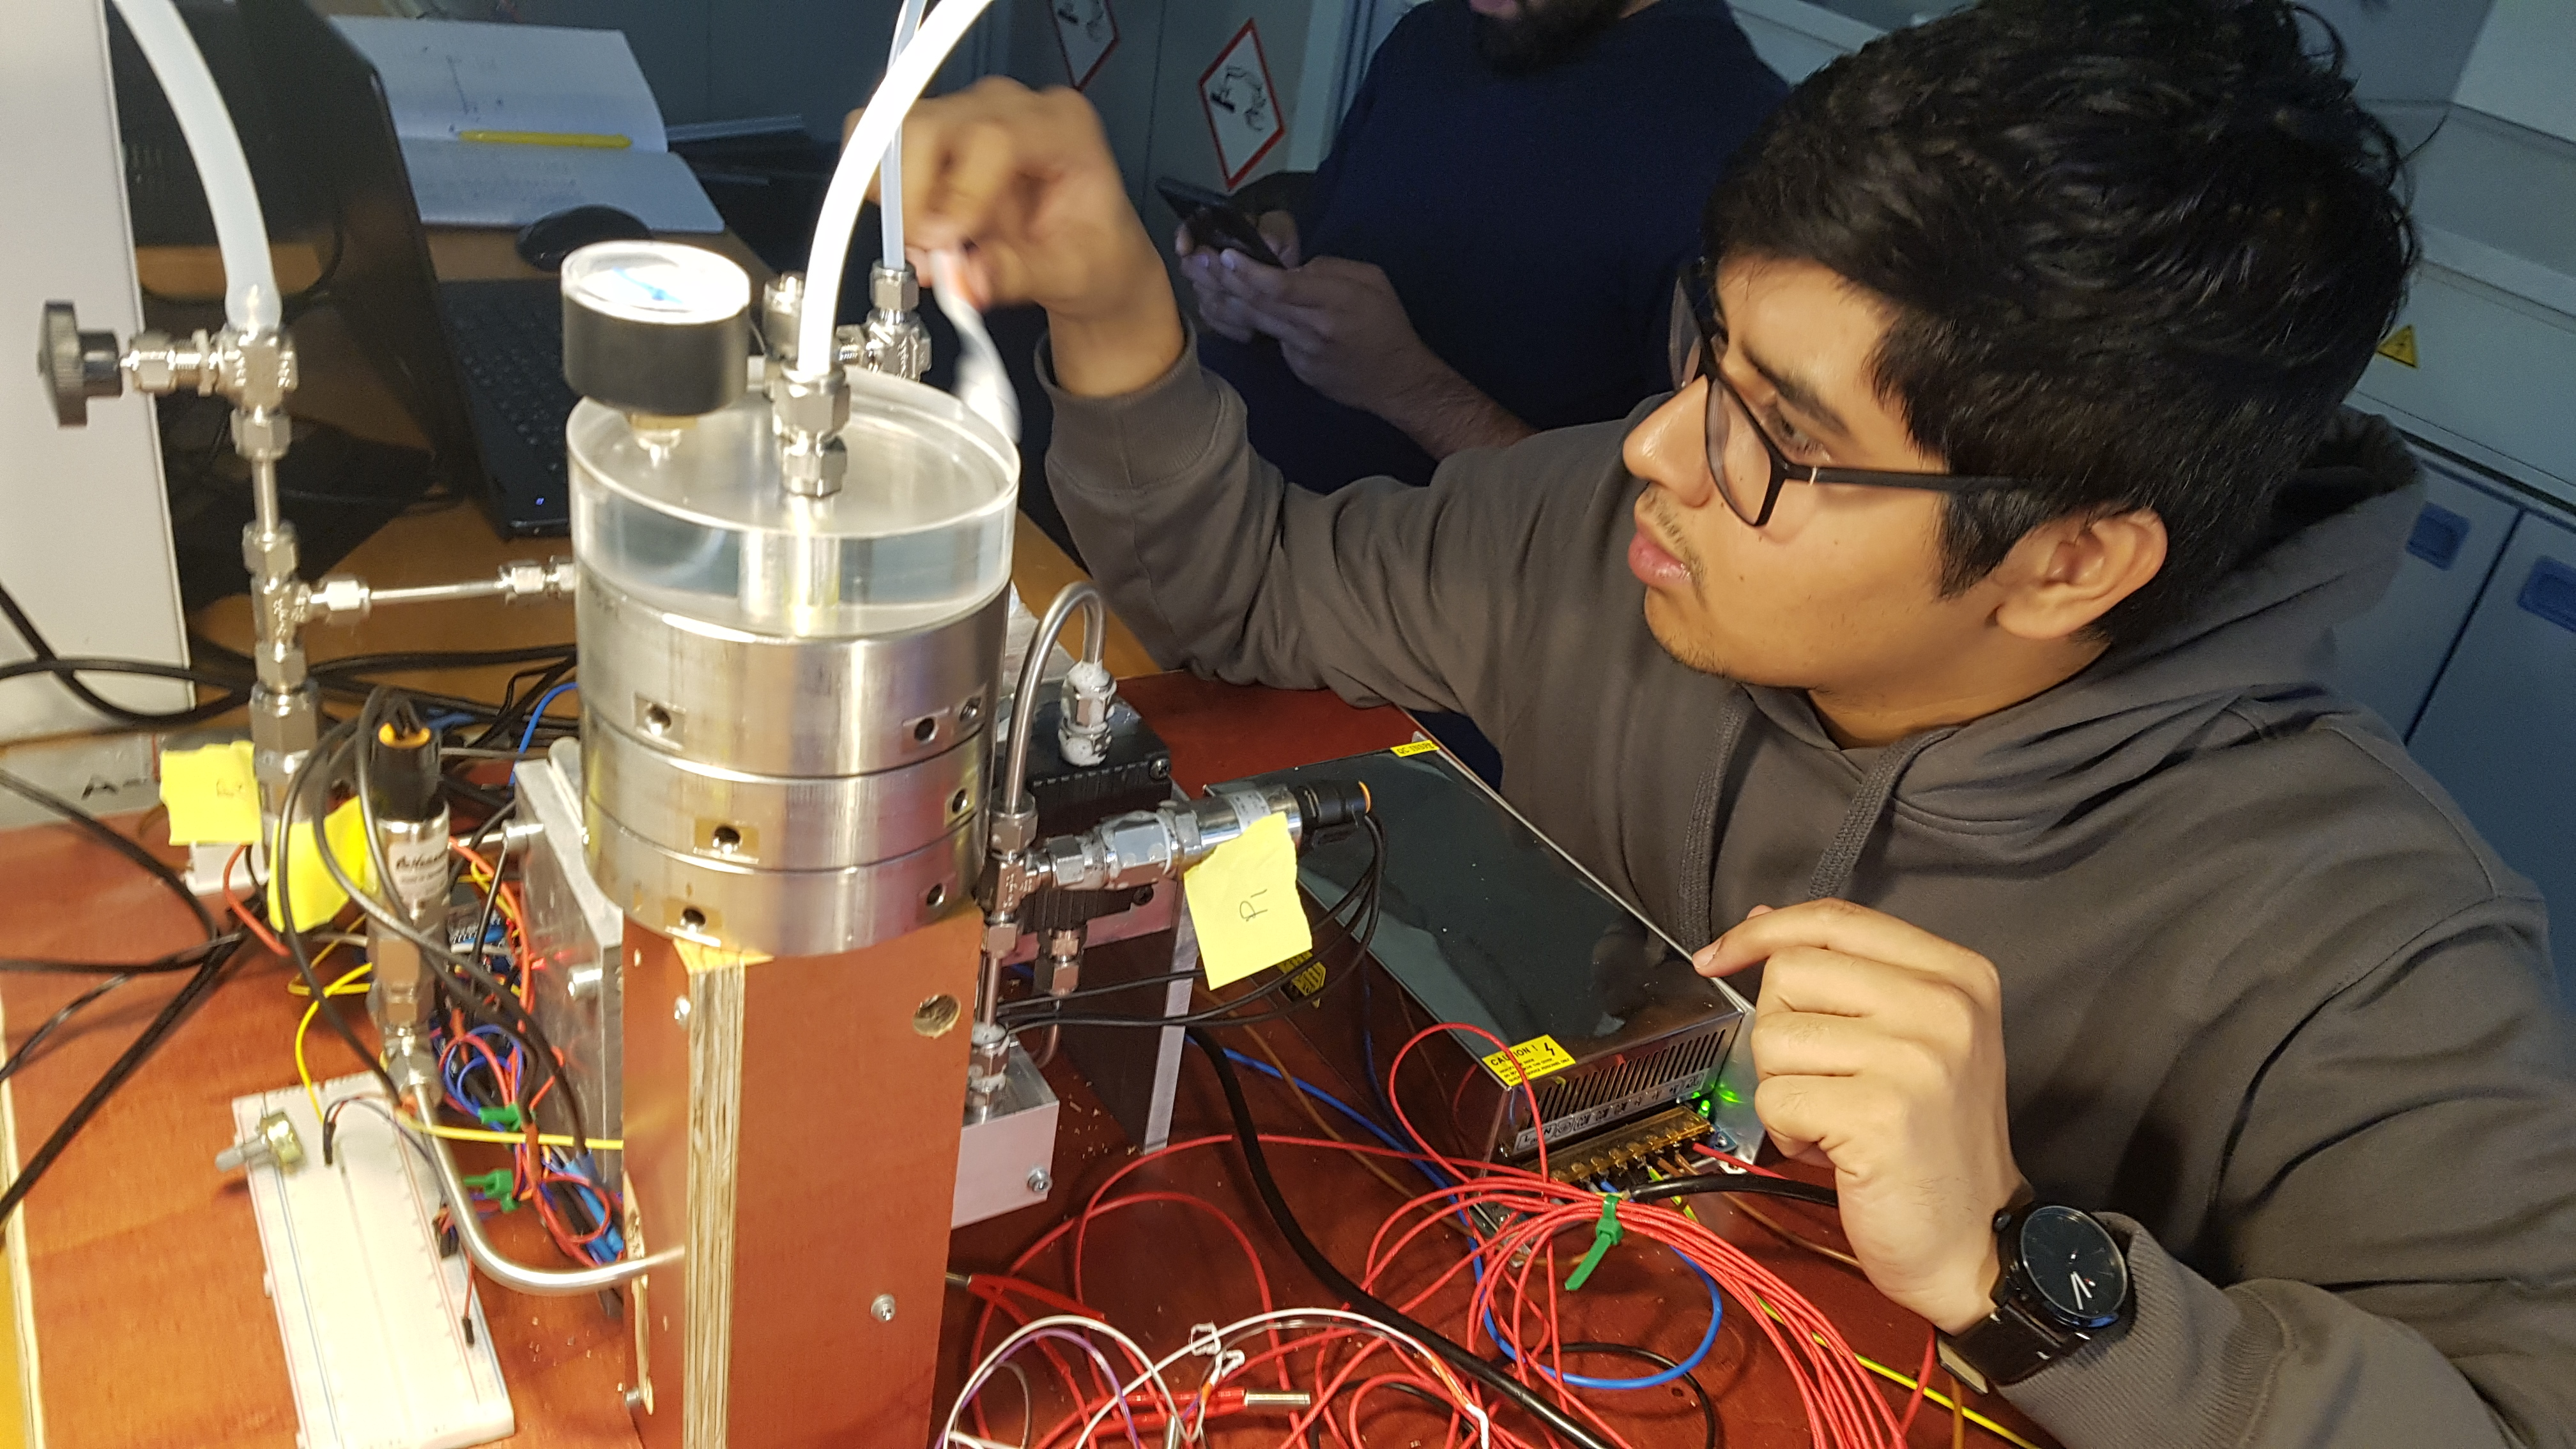
\includegraphics[width=0.9\linewidth]{images/mywork/Sprint2/Leaktest.jpg}
  \captionof{figure}{Leak test with bubbles}
  \label{fig:leaktest}
\end{minipage}%
\begin{minipage}{.5\textwidth}
  \centering
  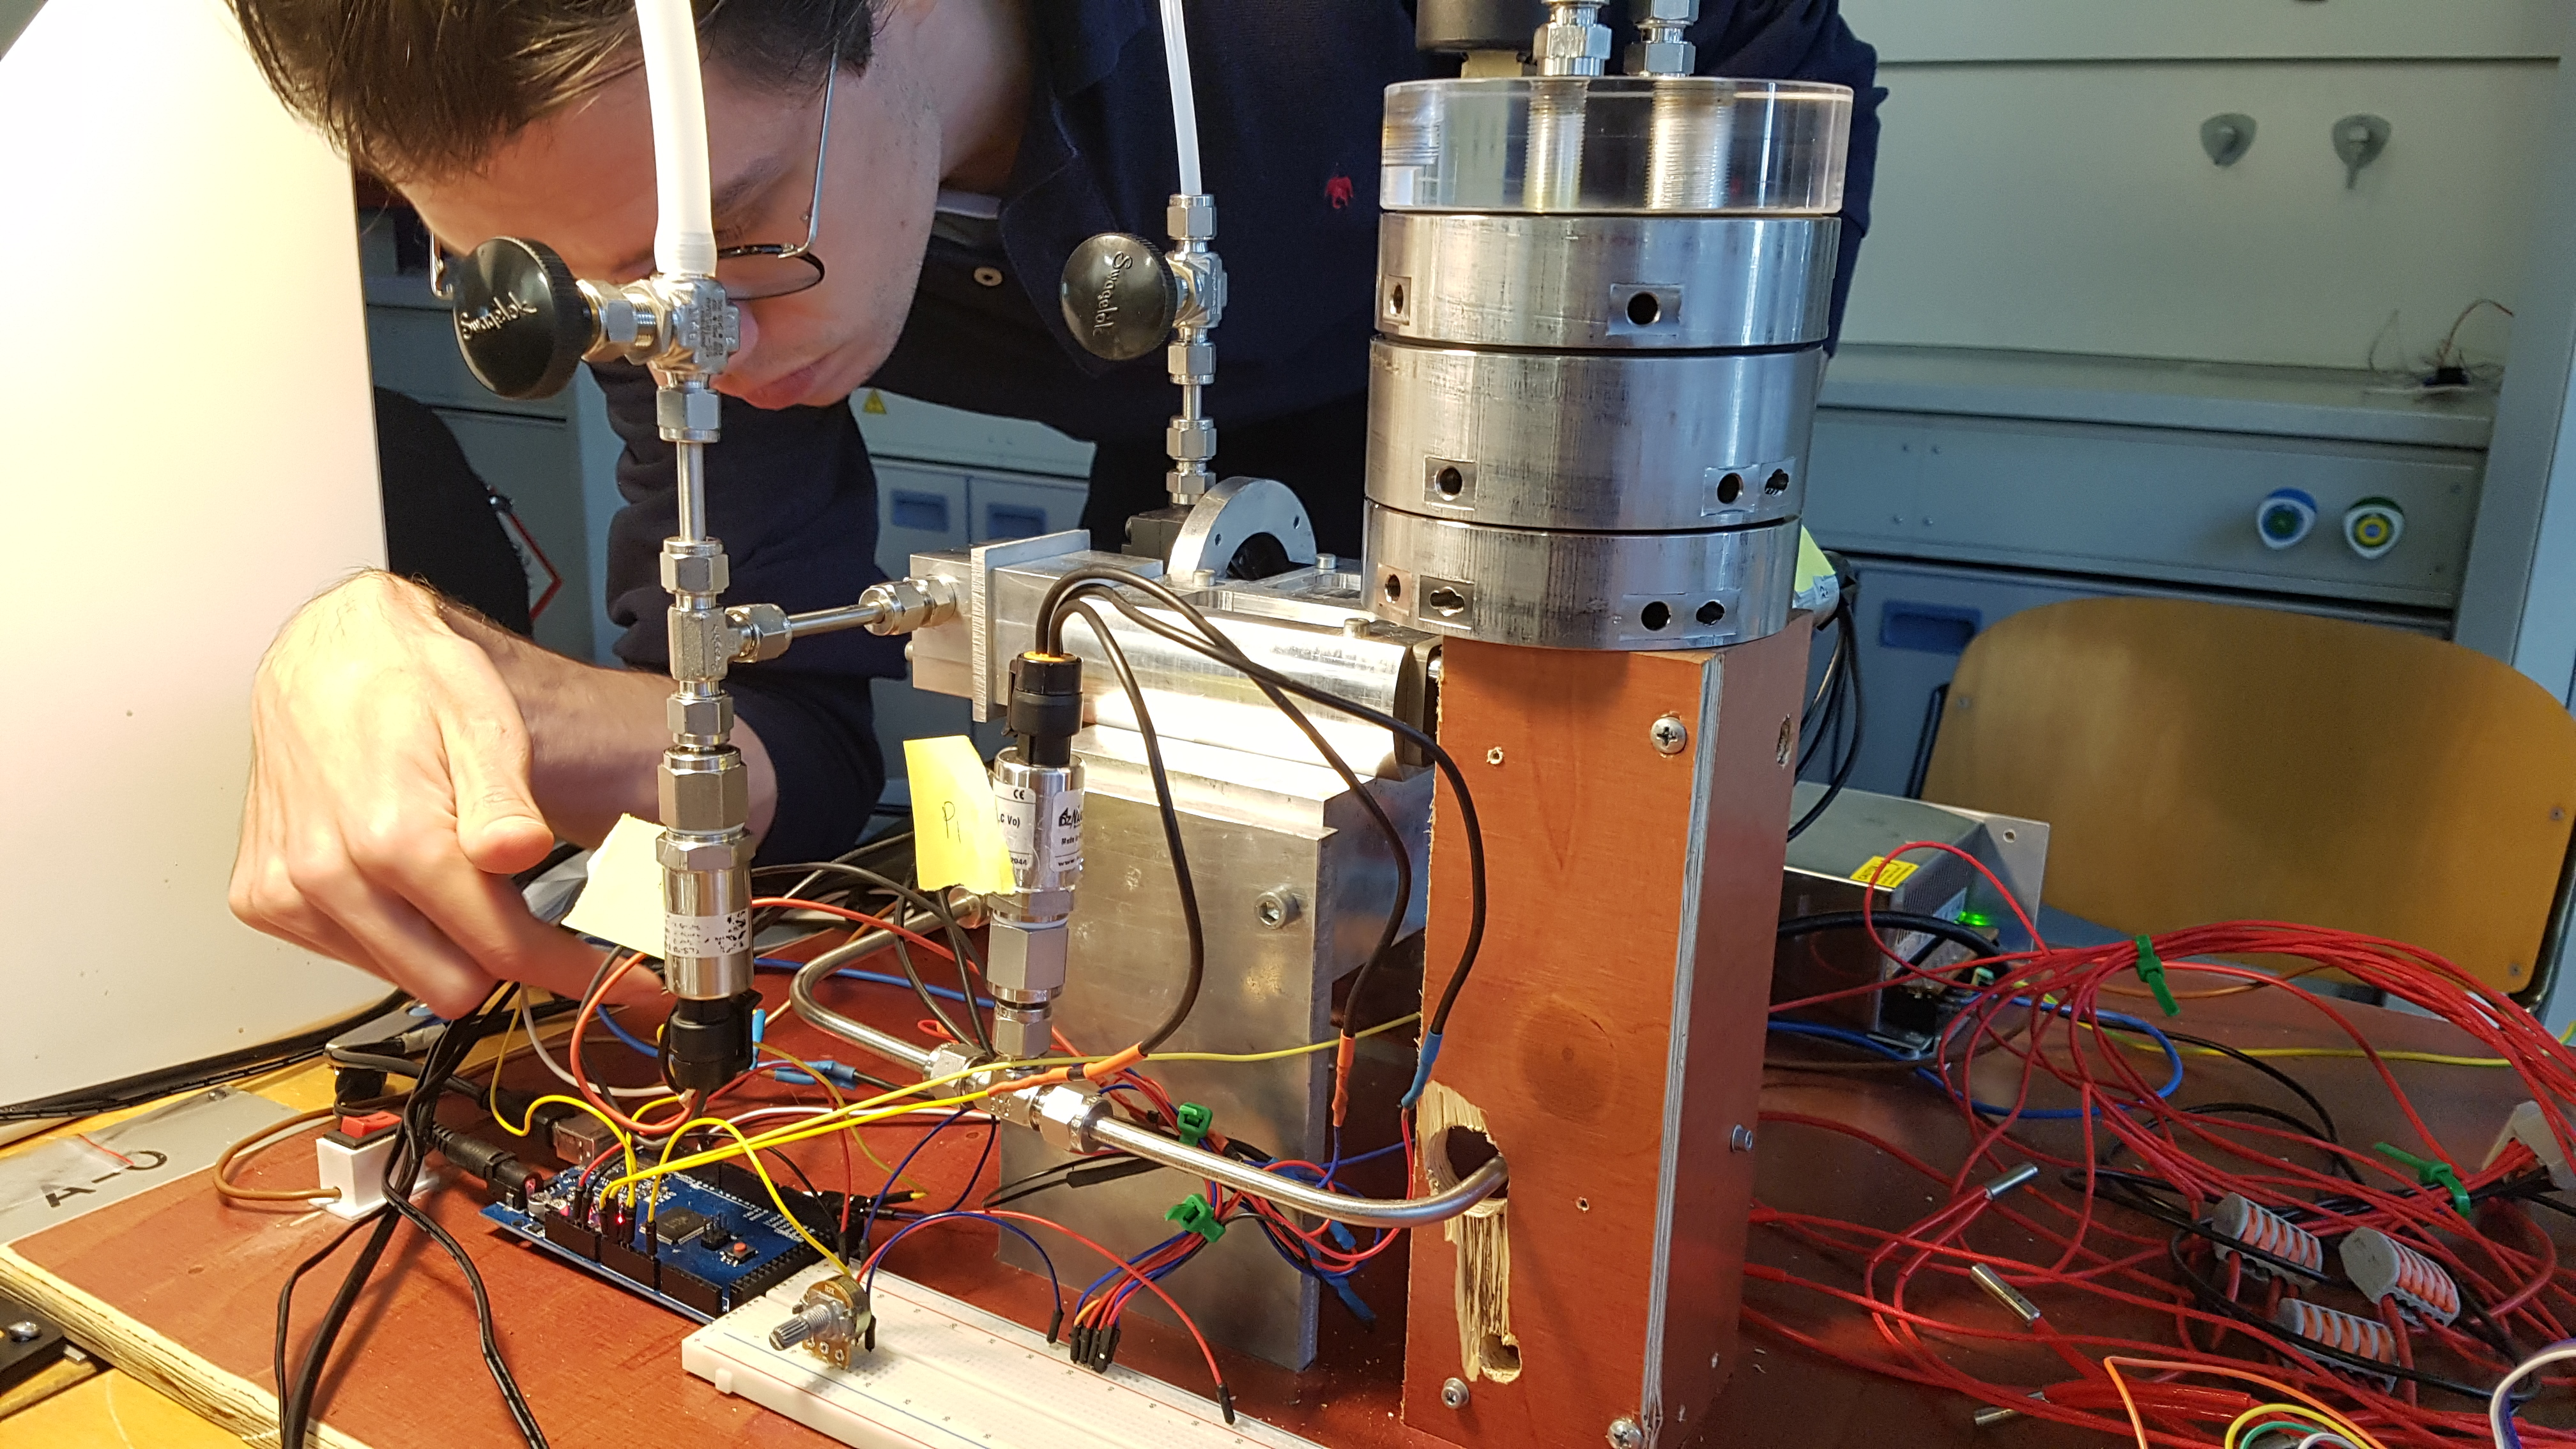
\includegraphics[width=0.9\linewidth]{images/mywork/Sprint2/desorbcheck.jpg}
  \captionof{figure}{Pressure sensor check}
  \label{fig:desorber}
\end{minipage}
\end{figure}


\subsubsection{Running DAC V1.1 system}

During the second half of the sprint, once the absorber and desorber subsystems of the DAC system V1.1 is complete. The system components were connected together using silicon connecting pipes so that PEI can flow through the system. The fluid will be fed into the system using the collector bucket and then fluid shall be pumped across the system using the PEI pump. Water was passed through the system and the observations made in the system in the Section \ref{sec:watertest}. 
\bigbreak



\subsection{Sprint 3 - $14^{th}$ October to $4^{th}$ November}
\label{sec:sprint3}

Sprint 3 proved to be one of the toughest parts of the internship since it involved a lot of messy work since we were working with PEI and heartbreak since mid-sprint our system broken down. The reasons for the system breakdown shall be elaborated more in the Section \ref{sec:breakdown}. On running the system continuously for hours, we could make some quite interesting observations which can be seen in Section \ref{sec:obs}.  


\subsection{Sprint 4 - $4^{th}$ November - $25^{th}$ November}
\label{sec:sprint4}

During the $4^{th}$ phase of the internship, we laid the foundations for the DAC V2.0 system. We had addressed the issues we faced while running the DAC V1.1 system for long hours as elaborated in Section \ref{sec:breakdown}. We also changed the material used for prototyping and the type of the manufacturing the prototype as well which is from 3D printing to SLS printing. 

\subsubsection{Design changes}
In order to rectify the geometry mistakes we changed the geometry of some of the DAC components. The design of the components were changed in order to accommodate these changes which will be elaborated more below :

\begin{itemize}
    \item \textbf{Manifold :} in-order to make the flow uniform and make sure that all the PEI that has absorbed $CO_2$ is distributed uniformly, the internals of the manifold is made in the form of a cylinder than its cuboidal shape. The internal diameters of the manifold nozzles were also changed to 6mm diameter. As seen in Figure \ref{fig:newmani}, the new manifold has a swagelok connection to the manifold that supplies the TEPA inlet, unlike in the old manifold as seen in Figure \ref{fig:oldmani}.
    
    
        \begin{figure}[H]
        \centering
        \begin{minipage}{.5\textwidth}
        \centering
        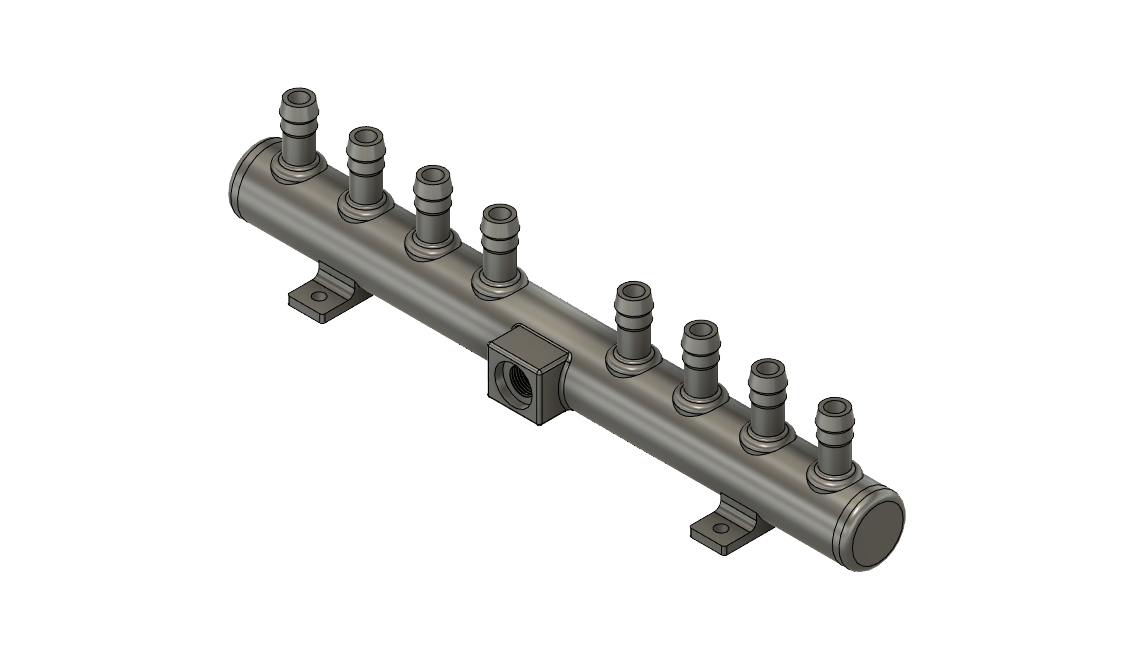
\includegraphics[width=\linewidth]{images/mywork/Sprint4/Manifold_main.png}
        \captionof{figure}{DAC V2.0 Manifold}
         \label{fig:newmani}
    \end{minipage}%
    \begin{minipage}{.5\textwidth}
        \centering
        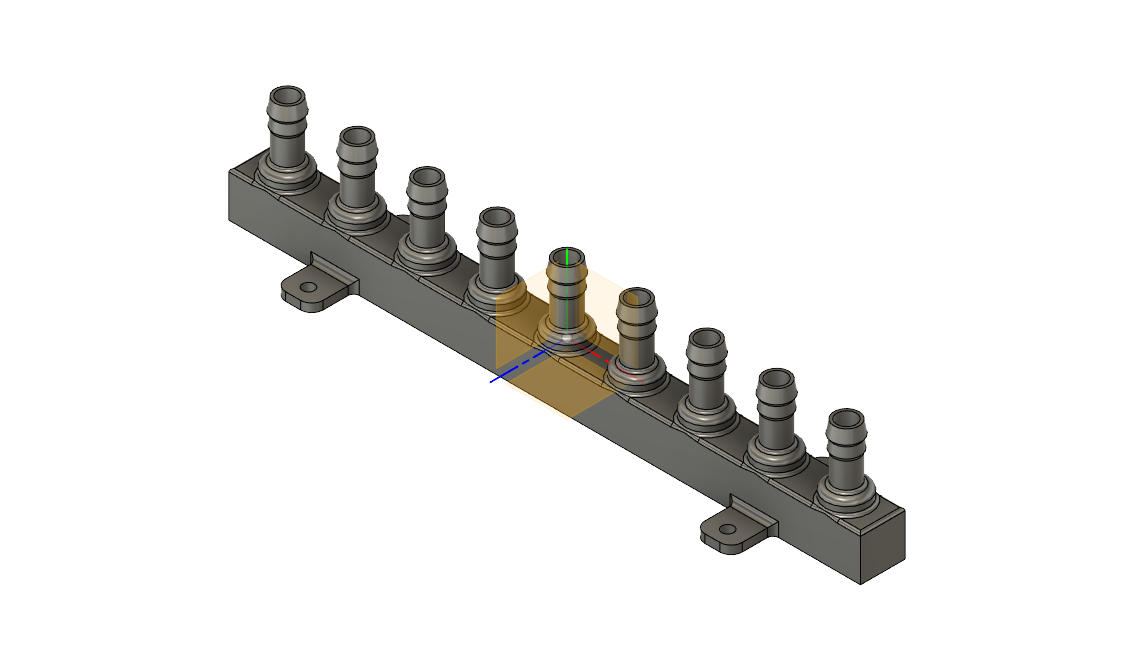
\includegraphics[width=\linewidth]{images/mywork/Sprint4/Manifold_old.png}
        \captionof{figure}{DAC V1.1 Manifold}
        \label{fig:oldmani}
    \end{minipage}
    \end{figure}
    
    \item \textbf{Collector :} In order to address the undesired PEI flowing out of the collector. We changed the outlet into a bent nozzle as seen in Figure \ref{fig:newcoll}. I wanted to give more support for the DAC channel plates and hold it with a grip like the DAC distributor system holds it together. This was done by creating slots which can keep the . By doing so, the DAC channels will be held in place rather than in an haphazard manner like in the last system where we had to drill holes on the PMMA sheets and added nails to keep them in place. 
    
    \begin{figure}[H]
        \centering
        \begin{minipage}{.5\textwidth}
        \centering
        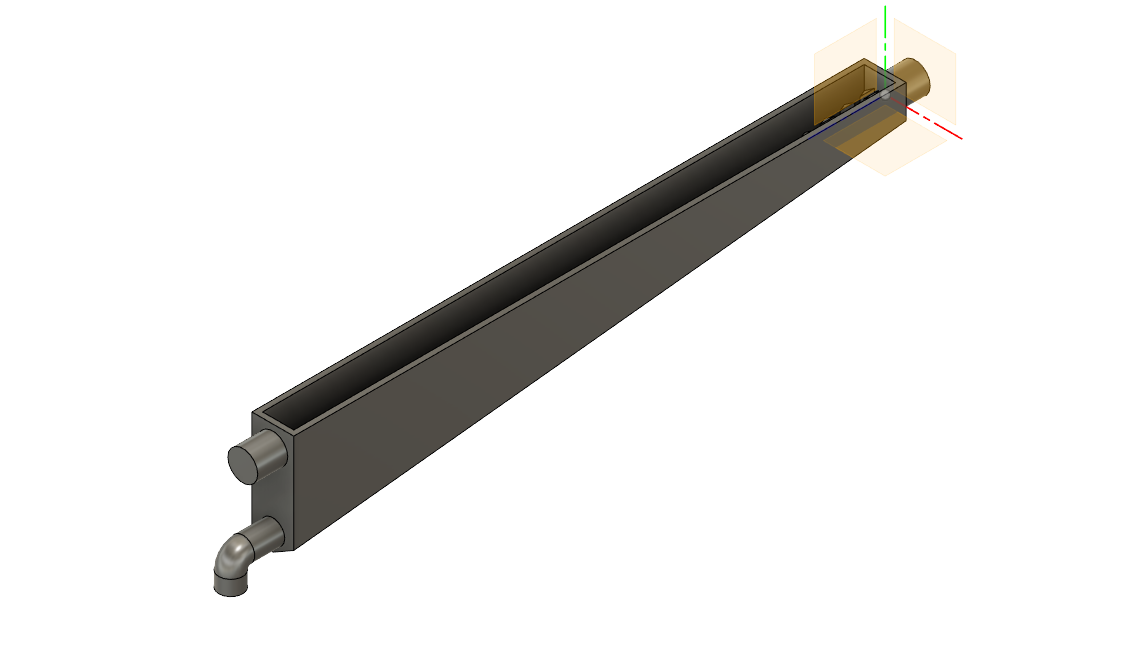
\includegraphics[width=\linewidth]{images/mywork/Sprint4/Collector_main.png}
        \captionof{figure}{DAC V2.0 Collector}
         \label{fig:newcoll}
    \end{minipage}%
    \begin{minipage}{.5\textwidth}
        \centering
        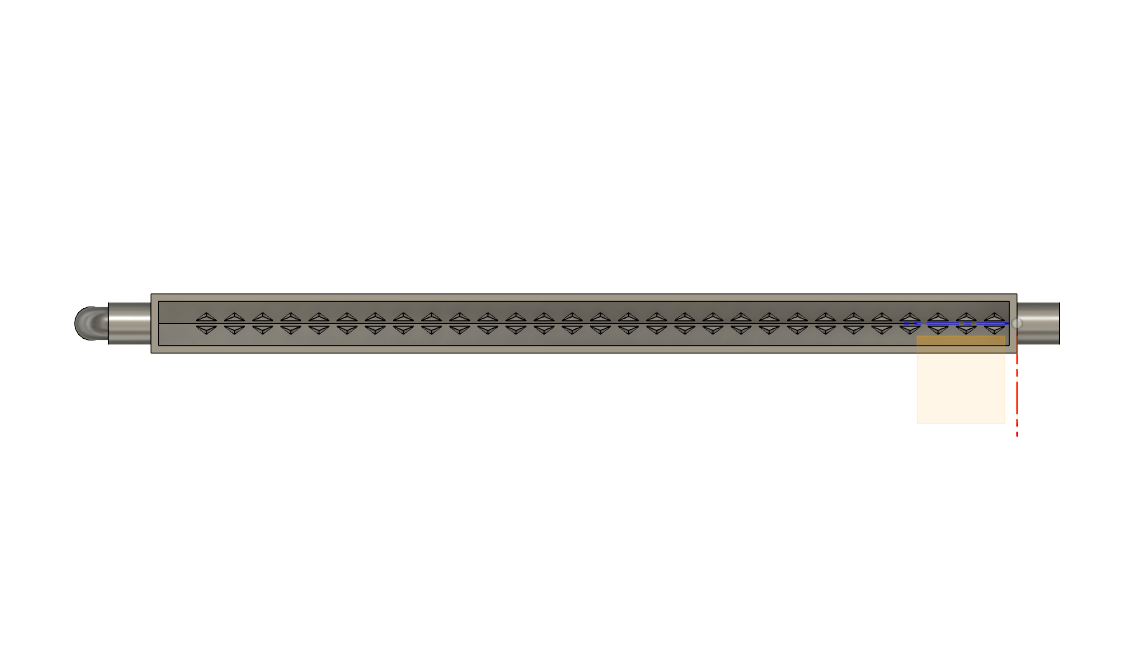
\includegraphics[width=\linewidth]{images/mywork/Sprint4/Collector_new_top.png}
        \captionof{figure}{DAC V2.0 Collector top view}
        \label{fig:newcolltop}
    \end{minipage}
    \end{figure}
    
    
    \begin{figure}[H]
        \centering
        \begin{minipage}{.5\textwidth}
        \centering
        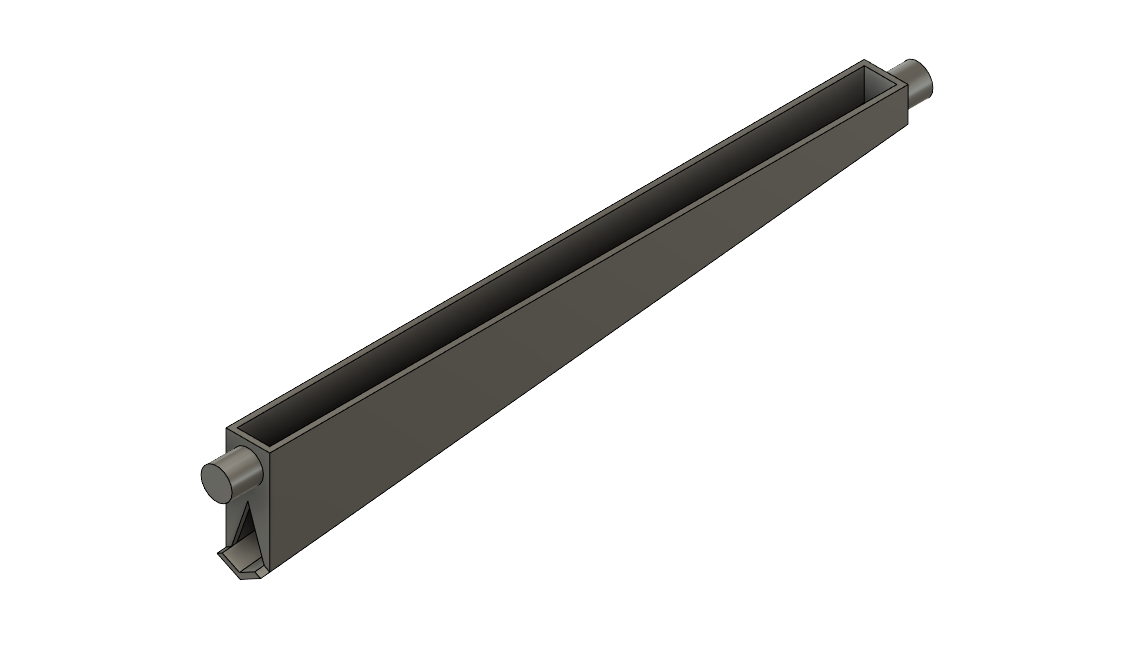
\includegraphics[width=\linewidth]{images/mywork/Sprint4/Collector_old.png}
        \captionof{figure}{DAC V1.1 Collector}
         \label{fig:oldcoll}
    \end{minipage}%
    \begin{minipage}{.5\textwidth}
        \centering
        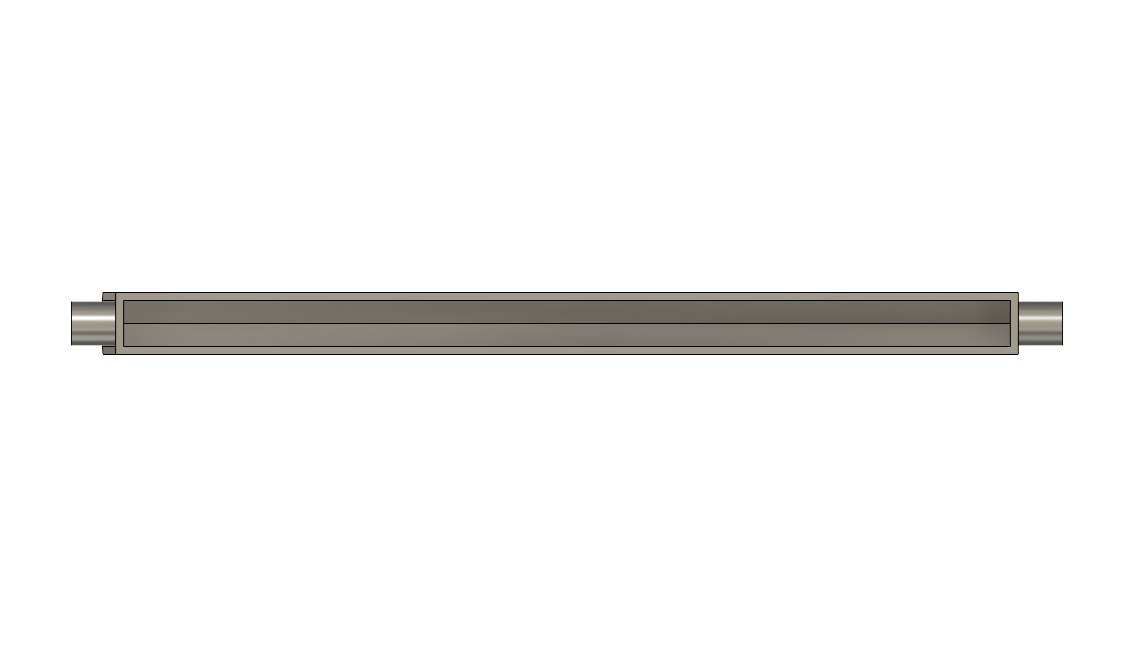
\includegraphics[width=\linewidth]{images/mywork/Sprint4/Collector_old_top.png}
        \captionof{figure}{DAC V1.1 Collector top view}
        \label{fig:oldcolltop}
    \end{minipage}
    \end{figure}
    
    
        Comparing Figure \ref{fig:newcoll} and Figure \ref{fig:oldcoll}, we can see the new nozzle extension in the new DAC V2.0 Collector. On observing Figure \ref{fig:oldcolltop} and Figure \ref{fig:newcolltop} we can see the extra slots added to hold the DAC polypropelene channels in place. It also eliminates the need for nails for fixing the polypropelene channels in place as in DAC system V1.1. 
        
        \item \textbf{Distributor :} The distributor had very less design changes and with respect to design. The old distributor design worked perfectly but in-order to make it better. The cross section of the distributor is changed from a cylindrical cross section to a rectangular cross-section for uniform distribution of TEPA or PEI as per Mr. Leonard Schrug's recommendations. The internal diameter was also changed to 6 mm. Since, the new prototyping method was using SLS method, I had made a M6 screw threaded hole so that after machining, the manufactures can clear all the pieces inside the chamber. Once we receive the distributors, we close the holes using M6 screws. 
        
        \begin{figure}[H]
        \centering
        \begin{minipage}{.5\textwidth}
        \centering
        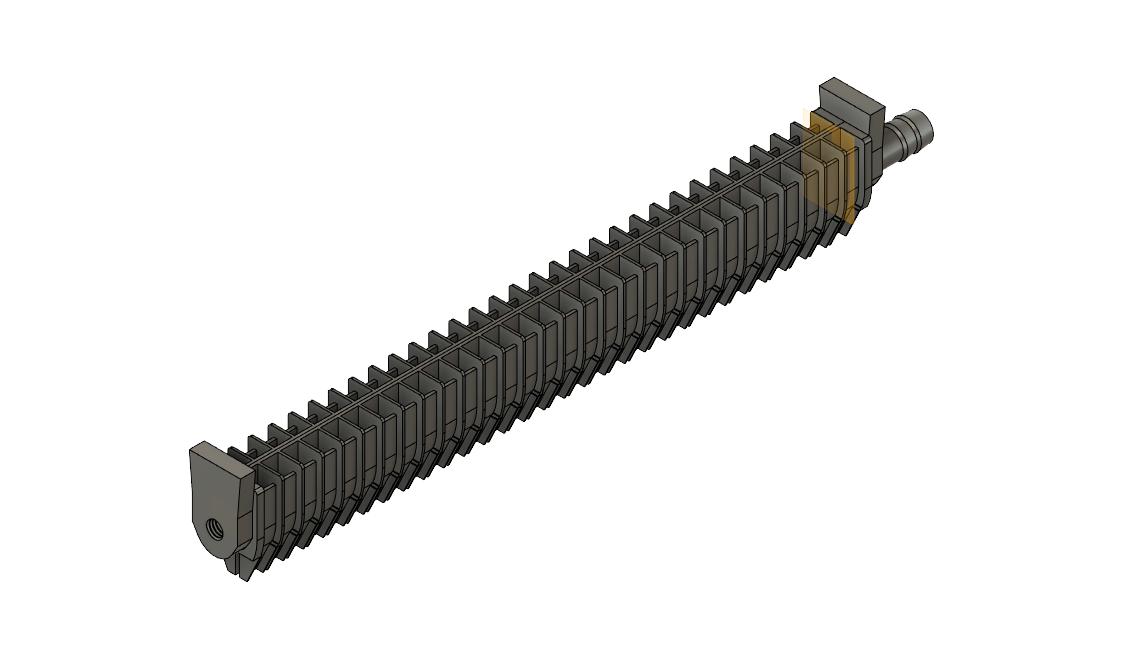
\includegraphics[width=\linewidth]{images/mywork/Sprint4/Distributor_main.png}
        \captionof{figure}{DAC V2.0 Distributor}
         \label{fig:2dis}
    \end{minipage}%
    \begin{minipage}{.5\textwidth}
        \centering
        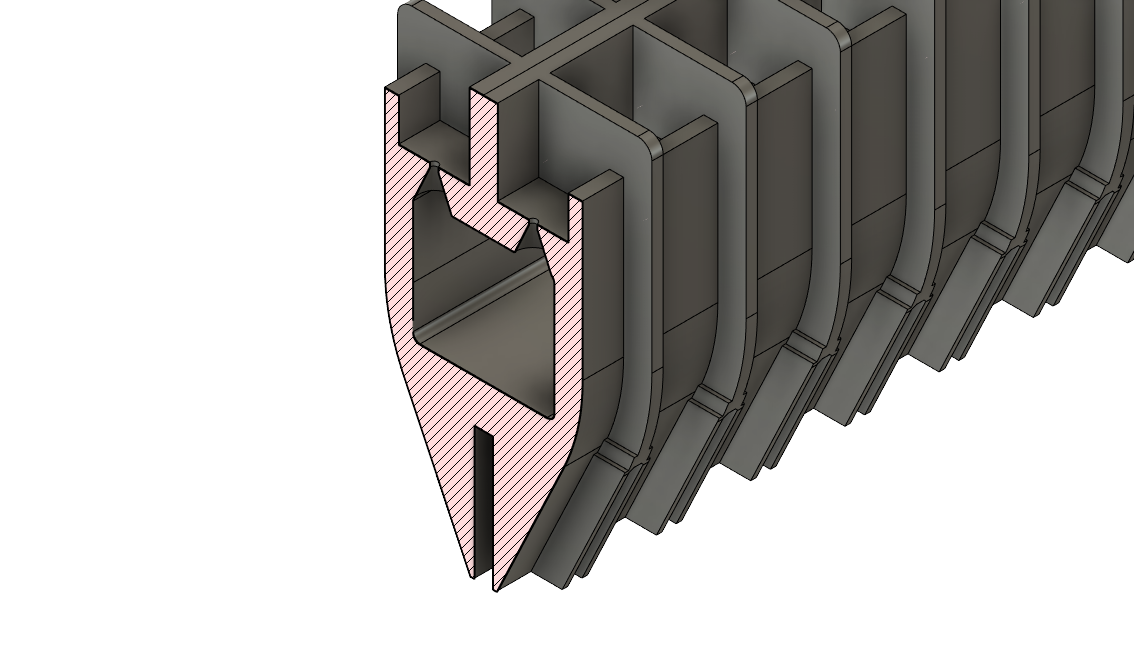
\includegraphics[width=\linewidth]{images/mywork/Sprint4/newdiscross.png}
        \captionof{figure}{DAC V2.0 Distributor cross section}
        \label{fig:2discross}
    \end{minipage}
    \end{figure}
    
    
    \begin{figure}[H]
        \centering
        \begin{minipage}{.5\textwidth}
        \centering
        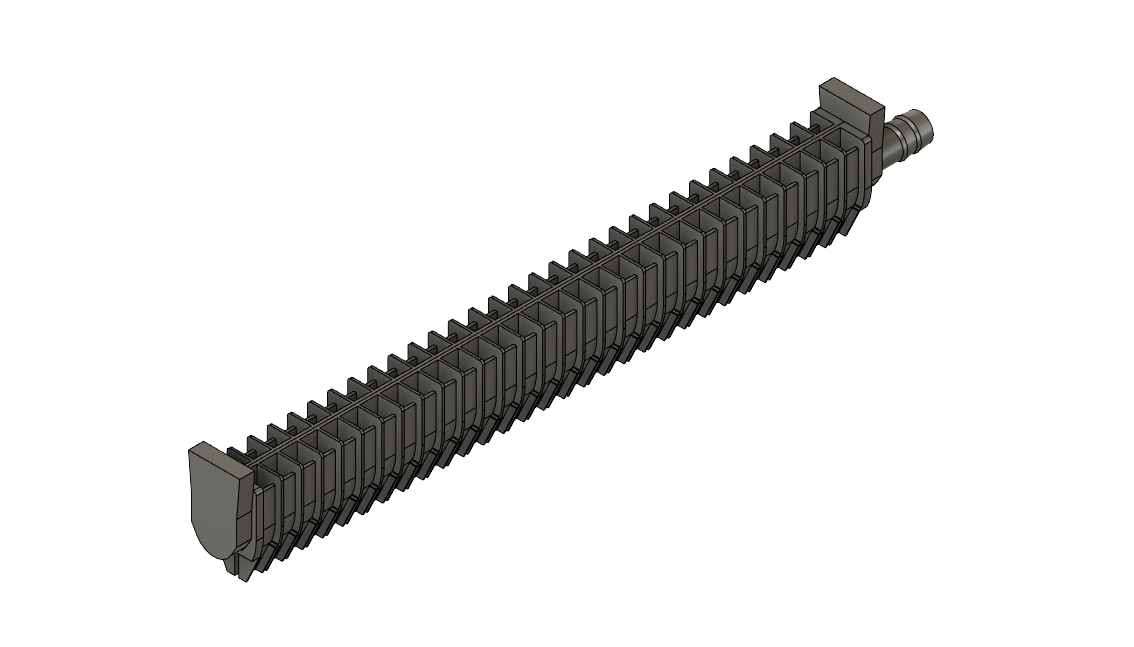
\includegraphics[width=\linewidth]{images/mywork/Sprint4/Distributor_old.png}
        \captionof{figure}{DAC V1.1 Distributor}
         \label{fig:1dis}
    \end{minipage}%
    \begin{minipage}{.5\textwidth}
        \centering
        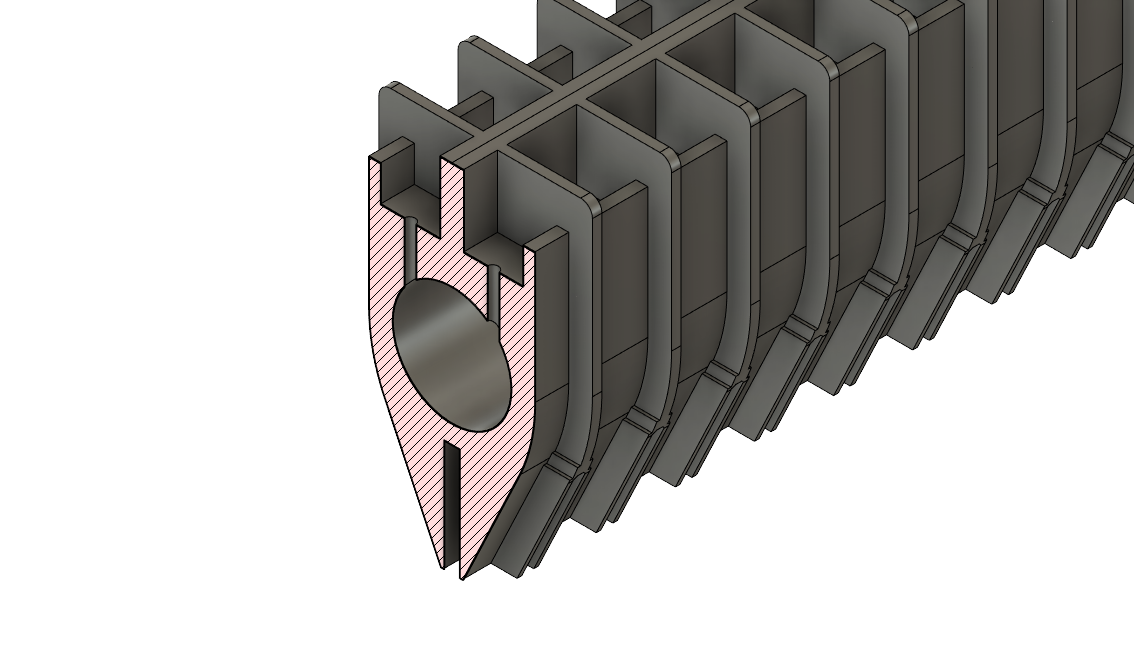
\includegraphics[width=\linewidth]{images/mywork/Sprint4/olddiscross.png}
        \captionof{figure}{DAC V1.1 Distributor cross section}
        \label{fig:1discross}
    \end{minipage}
    \end{figure}
    
    
    As seen in Figure \ref{fig:2dis}, the new distributor component has a M6 screw thread hole. The comparision of the cross sections difference between the new and the old design can be seen in Figure \ref{fig:2discross} and Figure \ref{fig:1discross}. In the above Figures, we can also see that the nozzle designs have been changed as well for better distribution and smaller nozzle diameter. 
    
\end{itemize}

\subsubsection{Material and production changes}

We have seen in Section \ref{sec:hotpei} that hot PEI reacts with the 3D printing material PLA. Hence, this caused many DAC components like the distributors, the nozzles of the collector bucket and manifold to break due to chemical degradation. This was later confirmed by Wino Spix when he reacted hot PEI with PLA material in a stand alone environment. In order to overcome this issue, we looked into various other ways of prototyping and thanks to Leanord's recommendation. It was decided to go for SLS printing with the prototype material being nylon. We tested the SLS material first to see its reaction with TEPA since it is known that TEPA is more reactive in nature. Besides some discoloration due to the porus nature of nylon. The material was still intact after hours of exposure to TEPA. Hence, prototyping was done by SLS printing using nylon material.    


\subsubsection{Component changes}

It was decided to remove or change some components of the DAC system in order to improve the system's efficiency or make it easier to see the process occurring. Some of the changes that we have done in for the new DAC V2.0 system are as follows : 

\begin{itemize}
    \item \textbf{LIS fabricated compressor :} In DAC V1.1 system, we had used a compressor system that was manufactured by the previous LISForce team but as we seen in Section \ref{sec:faultycomp} and in Figure \ref{fig:psensor} that the compressor system couldn't meet the desired pressure of 50 bar. Hence, the compressor system was removed and a entirely new vacuum pump is used to maintain vacuum conditions in the new DAC desorber system. 
    
    \item \textbf{Si tubing :} The Si tubing in the DAC V1.1 system was removed and decided to implement PTFE tubing for the flow of TEPA/PEI across the various DAC components. It is known that PTFE tubes are more robust and can handle high temperatures as well. Thereby making it an ideal candidate for the system. 
    
    \item \textbf{Desorber column:} In Section \ref{sec:faultycomp} it is covered that the old desorbtion column can be seen in Figure \ref{fig:leaktest} and Figure \ref{fig:desorber}. This desorber had many issues such as moving due to vibrations of the compressor and PEI pump system which is elaborated in Section \ref{sec:breakdown}. In order to combat this issue and to make the system more isolated and transparent to see the distillation and desorbtion process occuring. A stainless steel distillation column is ordered from AliExpress and will be placed seperately from the whole DAC system. This can be seen in the picture below in Figure \ref{fig:discol}.
    
    \begin{figure}[H]
        \centering
        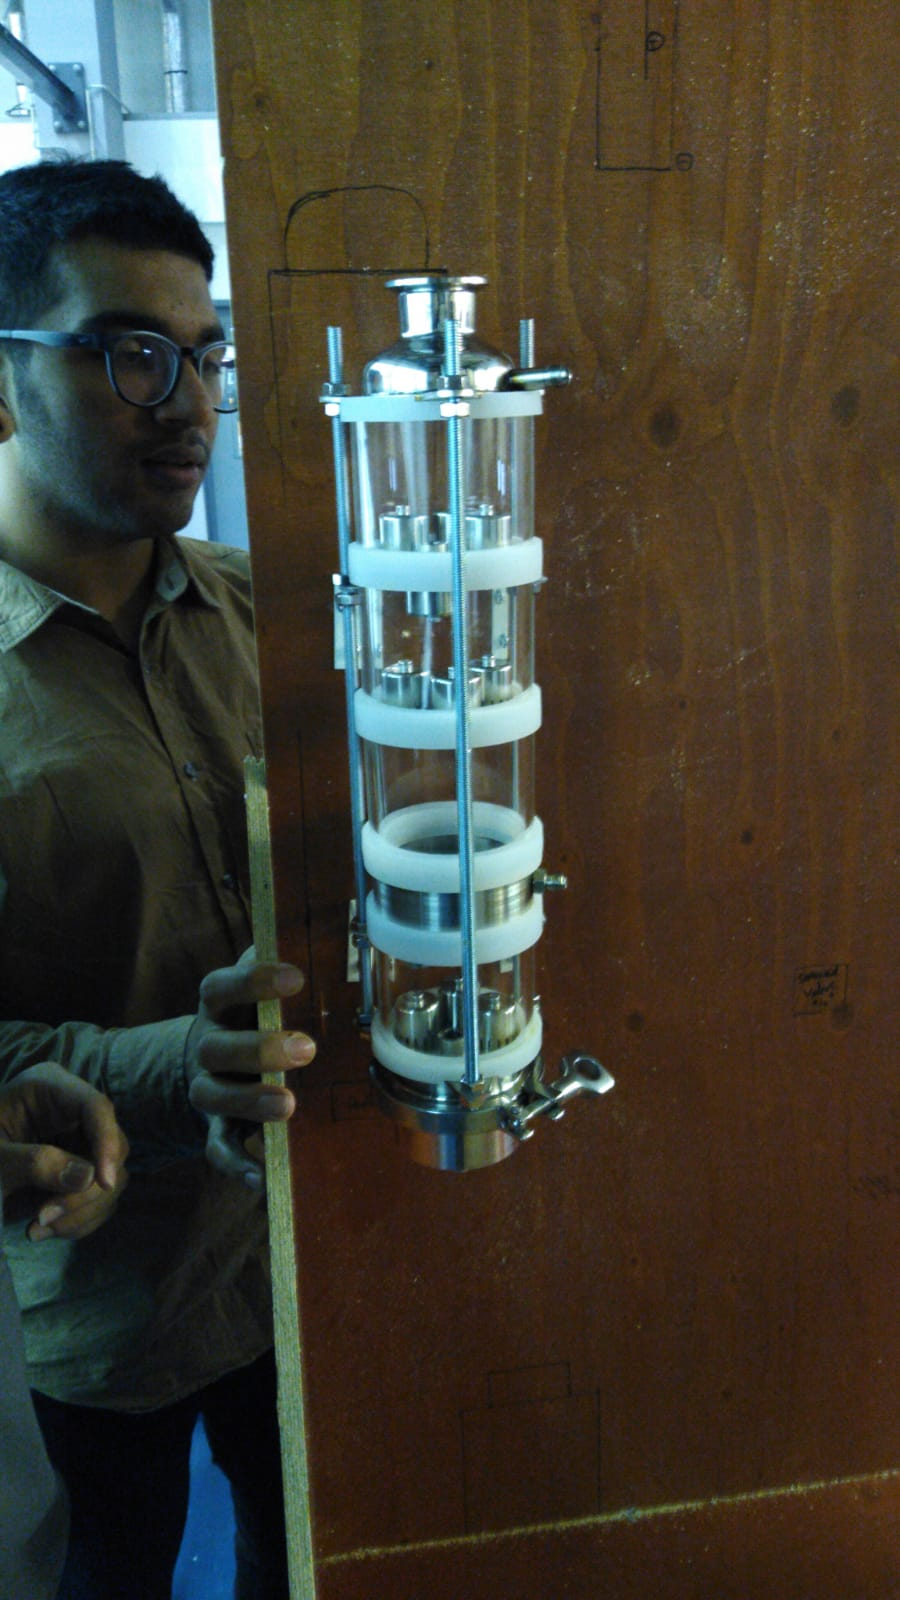
\includegraphics[scale = 0.25]{images/mywork/Sprint5/discol.jpg}
        \caption{DAC V2.0 distillation column}
        \label{fig:discol}
    \end{figure}

\end{itemize} 

\subsubsection{Process changes}

In order to combat some of the issues faced in the process stage in DAC V1.1 system some process changes were made. These changes were done inorder to increase the process efficiency and reducing the energy demand in the system. Some of the process changes made in the system are: 

\begin{itemize}
    \item \textbf{Straight finned tube: }In order to reduce the temperature of the hot PEI/ TEPA coming from the desorbtion unit to the DAC manifold (absorber). We use a straight fined tube that uses natural heat convection to cool down the hot PEI/ TEPA coming from the desorbtion unit to the manifold. Refer to Appendix \ref{ap:MATLAB} for the heat exchanger length calculation. 
    
    \item \textbf{Water pump: }We incorporate a water pump into the system to pump out the condensed water vapour from the flash tank after desorbtion. This is done so that we can get pure TEPA/ PEI from the system that is shown to have highest $CO_2$ absorbtion conditions as per previous studies done by Bart Ovaa \cite{Ovaa2019}. 

\end{itemize}
  



\subsection{Sprint 5 - $25^{th}$ November - $16^{th}$ December}
\label{sec:sprint5}

In the $5^{th}$ phase of the internship. We started the assembly of the DAC V2.0 system and incorporating the above component changes and material changes as well. Then in the later stages of the sprint we ran the system to check on it. The idea for the DAC V2.0 system to become more robust and run for much longer run times than before without stopping or refilling and making it a closed system. The system should also have a continuous $CO_2$ out-stream as well that can be fed to the Fluid Machinery subsystem to pump it out at 50 bar.

\subsubsection{Redesigning the DAC V2.0 collector bucket}

Due to the new polypropelene flow channels being not in the right dimensions due to the supplier fault. We had added the old polypropelene flow channels into the new system. However, it could be seen that the TEPA could leak out of the system. Hessel, one of the co - founders came up with a solution to it by making the collector bucket like a tray to collect all the TEPA flowing down the DAC flow channels thereby removing the need of the DAC collectors as well. However, for this system the Collectors will be left on the system to study about the individual flow of TEPA across the system. The component was fabricated by the LISForce and out of stainless steel. 

    \begin{figure}[H]
        \centering
        \begin{minipage}{.5\textwidth}
        \centering
        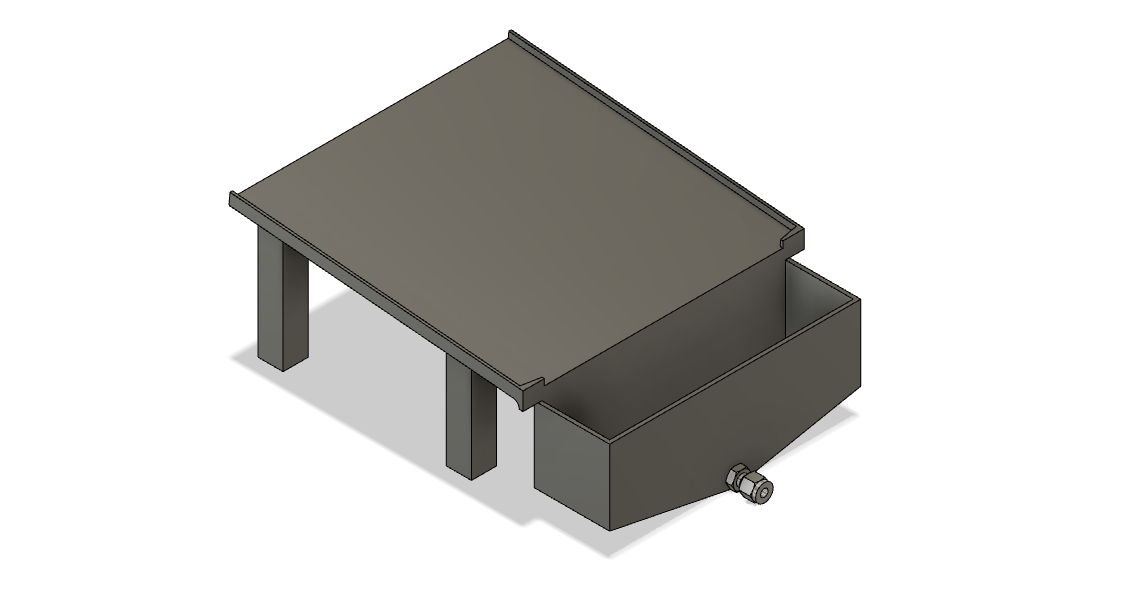
\includegraphics[width=\linewidth]{images/mywork/Sprint5/collbuc.png}
        \captionof{figure}{Collector bucket with tray}
         \label{fig:collbuctray} 
    \end{minipage}%
    \begin{minipage}{.5\textwidth}
        \centering
        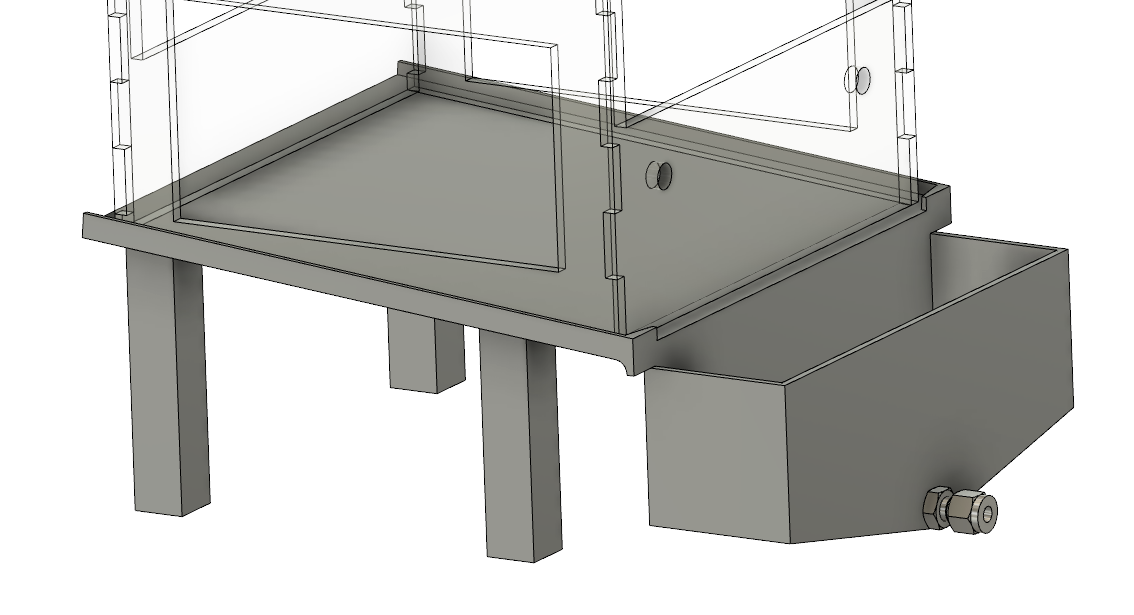
\includegraphics[width=\linewidth]{images/mywork/Sprint5/newpmma.png}
        \captionof{figure}{PMMA sheet correction}
        \label{fig:pmmatilt}
    \end{minipage}
    \end{figure}



In Figure \ref{fig:collbuctray}, we can see that since the the tray is placed at an angle to facilitate the flow of TEPA towards the collector bucket. So, the PMMA sheets of the DAC Absorber column must be modified inorder to stand on the tray which has an inclination of 5 \degree. Hence, we lasercut the PMMA sheets to remove the extra material and inclining the absorber column with an inclination of 5 \degree. The change in PMMA sheets can be seen in Figure \ref{fig:pmmatilt}.

\subsubsection{Assembling the DAC V2.0 Absorber}

The absorber column is easily assembled as we used the PMMA sheets for the column walls from the old system. However, we had order new PP sheets for the panels but due to some defect from the manufacturer's side. The flow channels weren't aligning with the distributor slots. In order to overcome this issue, we decided to use the old flow channels from DAC V1.1 system since it fits well with the new DAC V2.0 Distributors. In Appendix \ref{sec:setup2.0} refer the Figure \ref{fig:dacv2system}, where all the components are arranged in wooden board and named the "DAC V2.0 System".

\begin{itemize}
    \item \textbf{Connecting all the components: }In order to connect all the components together, PTFE and Swagelok tubing was used for the continuous flow of TEPA or PEI through the components. Since it highly heat resistant and PTFE tubing is used mostly since it will let us observe the flow of TEPA or PEI across the system. All the tubes are connected with Swagelok connections to make the tubing leak tight. Since we are working in vacuum conditions in the distillation column. 
    
    \item \textbf{The wooden board: }The desorbtion components such as the distillation column, the solenoid valves, the flash tank and macaroni are all clamped on to the wooden board using clamps and L brackets that were purchased from online and Gamma store respectively.The DAC V2.0 absorber rests on top of the wooden board's base.
    
    \item \textbf{The wiring: }The amount of wiring needed for the system was calculated similar to the method I used to estimate the size of the distributor hole in Appendix \ref{sec:holesize}. The length of the ground wire and live wire needed for the system is hence calculated and labeled for which component it should be connected to. All the electrical components are then connected to the DAC PCB which is shown in Figure \ref{fig:dacpcb} below. 
    
    \begin{figure}[H]
        \centering
        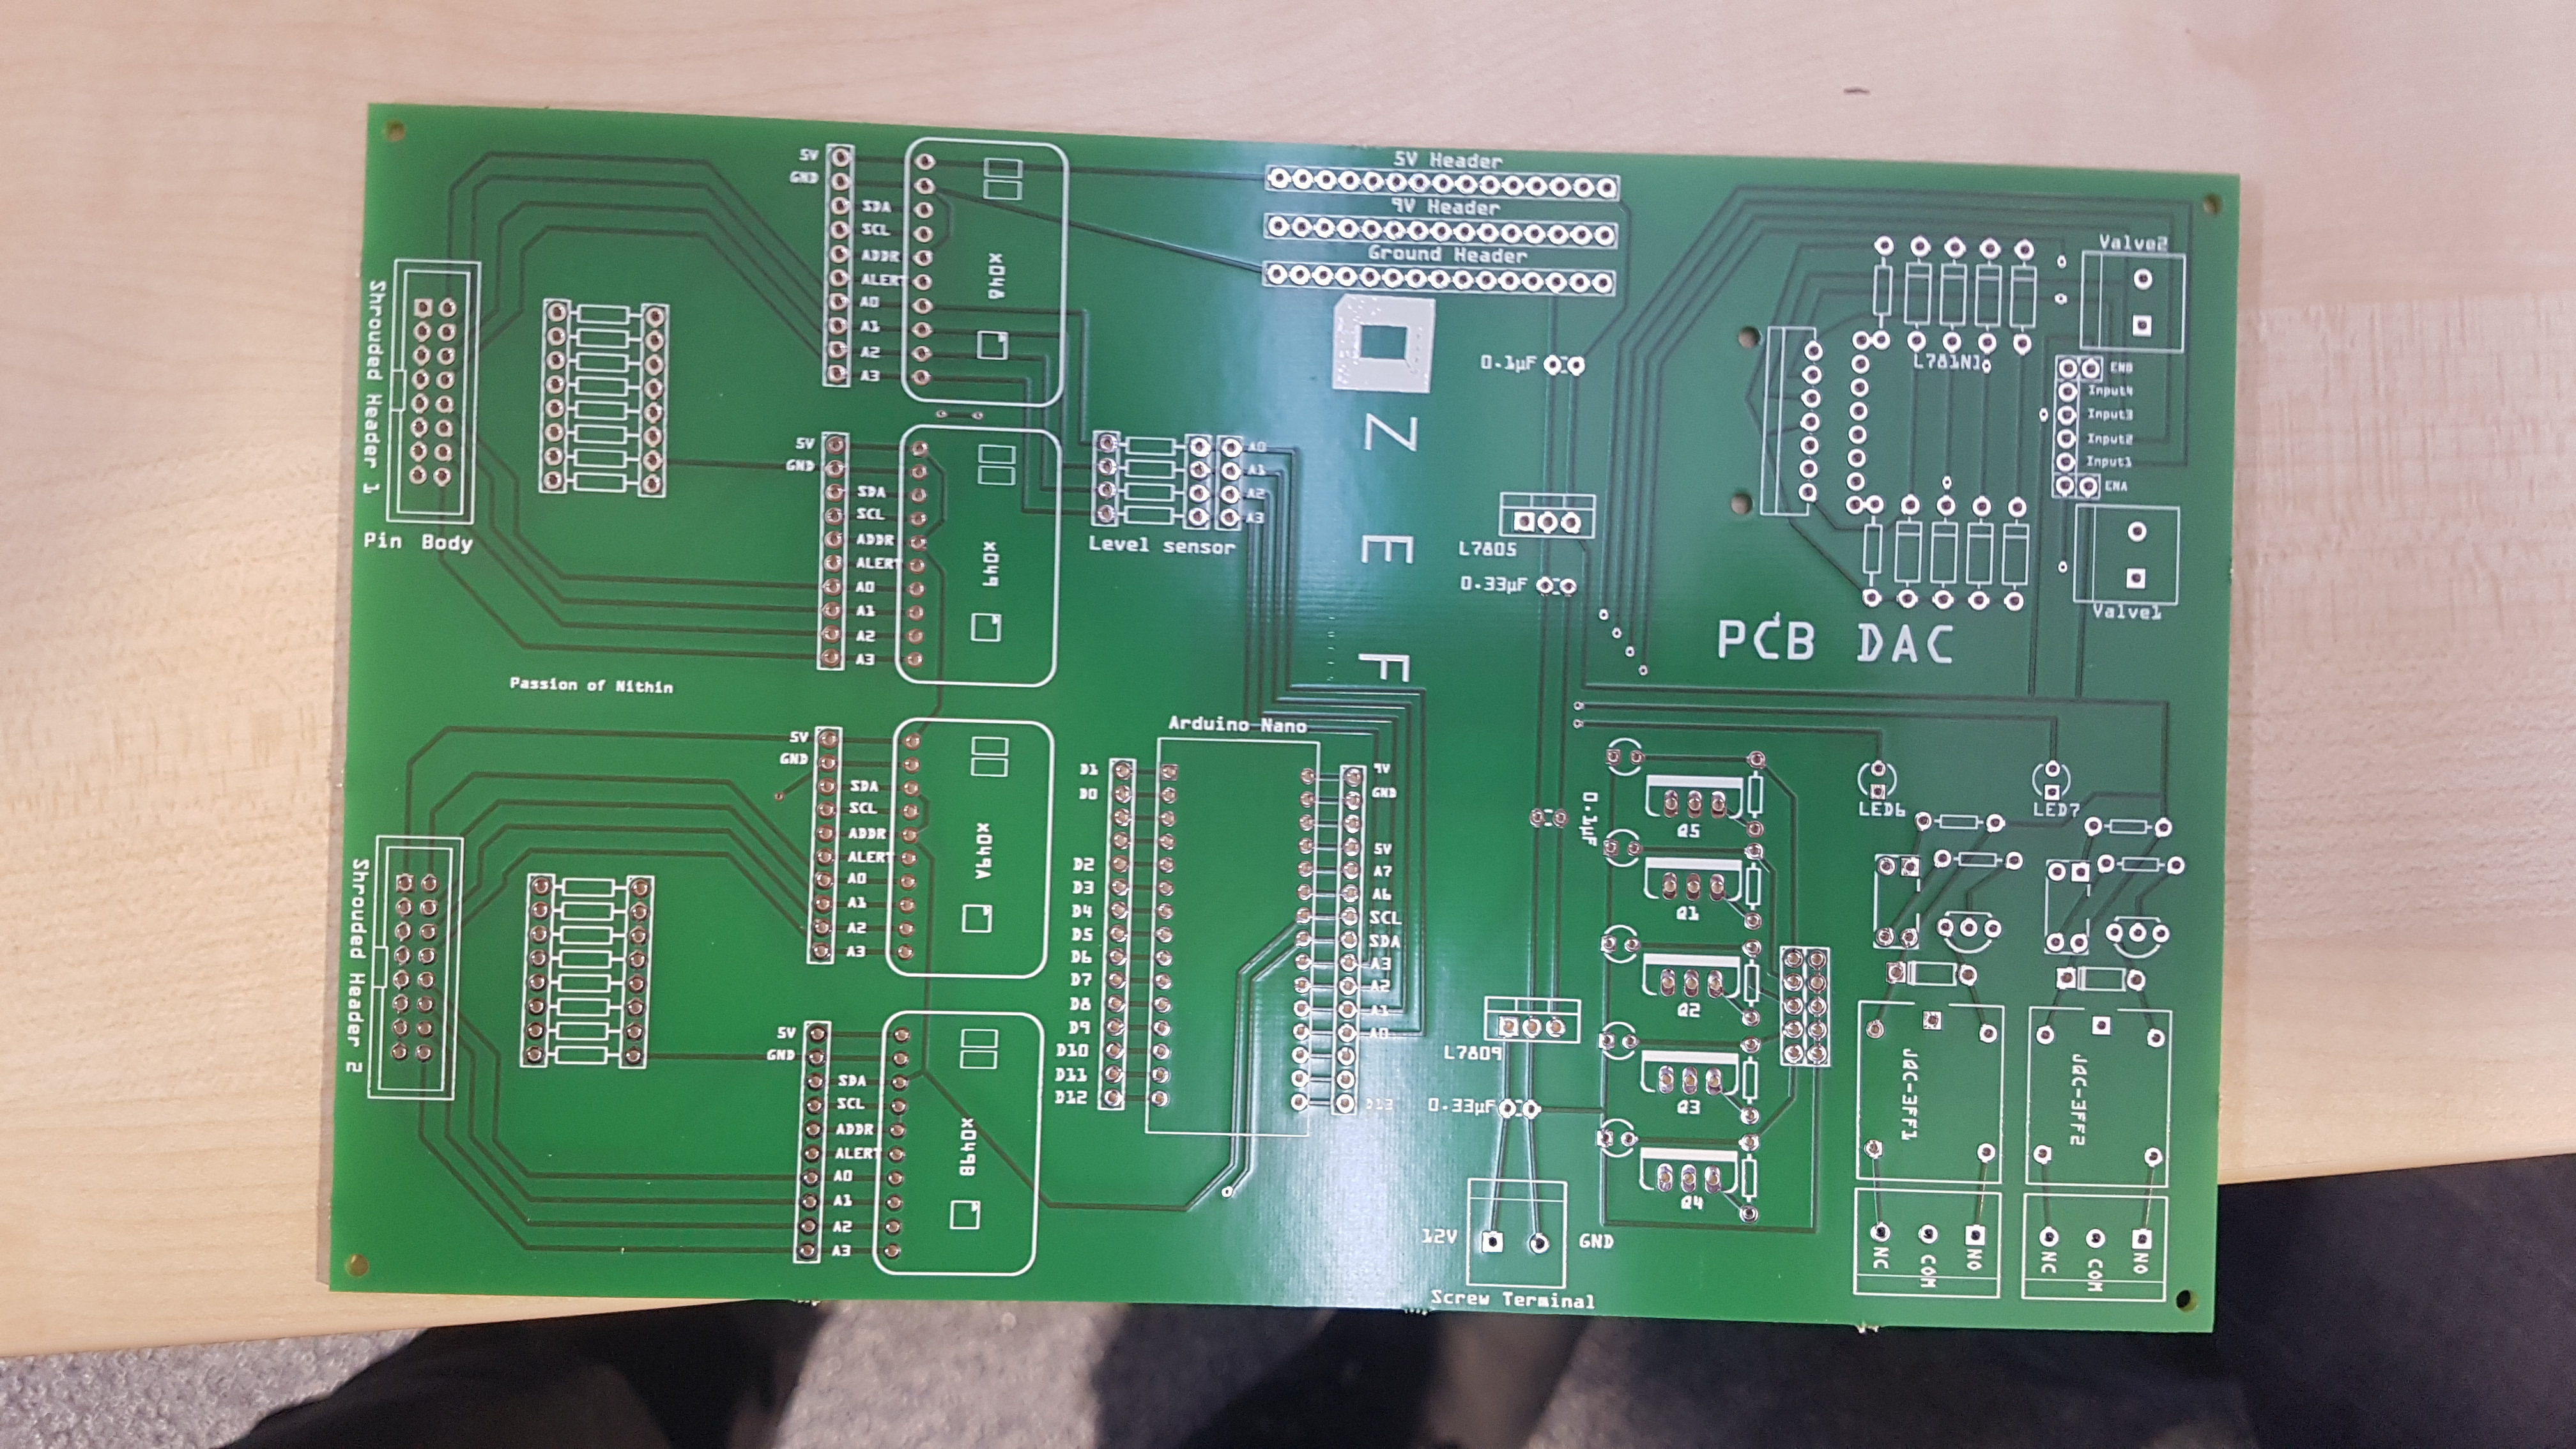
\includegraphics[scale = 0.09]{images/mywork/Sprint5/dacpcb.jpg}
        \caption{DAC printed circuit board (PCB)}
        \label{fig:dacpcb}
    \end{figure}
\end{itemize}

After the assembly of the whole DAC V2.0 system, vacuum leak testing had been done to check whether there were leaks in the system. This is done in order to make it a completely isolated desorbtion set-up. The results and observations of the vacuum leak testing is further elaborated in Section \ref{sec:DAC2.0leaks}.  
























